
%Generazione delle variabili che andranno a sostituire quelle del template 'HomePage.tex'
\newcommand{\documento}{\AdR}
\newcommand{\nomedocumentofisico}{AnalisiDeiRequisiti\_v1\_0\_0.pdf}
\newcommand{\redazione}{\TG \\ & \LC \\ & \CV \\ & \MM \\ & \SG \\ & \NC}
\newcommand{\verifica}{\TG \\ & \NC}
\newcommand{\versione}{1.0.0}
\newcommand{\approvazione}{\CV}
\newcommand{\uso}{Esterno}
\newcommand{\datacreazione}{27 novembre 2018} 
\newcommand{\datamodifica}{28 dicembre 2018}
\newcommand{\stato}{Approvato}
\newcommand{\destinateTo}{\TV, \\ & \RC, \\ & \II}

%TODO: non va elenco tabelle!
\def\TABELLE{true} % abilita - disabilita l'indice delle tabelle
\def\FIGURE{true}  % abilita - disabilita l'indice delle figure

\documentclass[a4paper,11pt]{article}

\usepackage{ifthen}
\usepackage[english,italian]{babel}
\usepackage[utf8]{inputenc}
\usepackage[T1]{fontenc}
\usepackage{float}
\usepackage{chapterbib}
\usepackage{graphicx}
\usepackage[a4paper,top=2.5cm,bottom=2.5cm,left=2.5cm,right=2.5cm]{geometry}

\PassOptionsToPackage{hyphens}{url}\usepackage[hyperfootnotes=false]{hyperref}
\hypersetup{%
	colorlinks=true,
	citecolor=black,
	linkcolor=black,
	urlcolor=blue
}

\usepackage{enumitem}
\usepackage{eurosym}
\usepackage{booktabs}
\usepackage{fancyhdr}
\usepackage{totpages}
\usepackage{tabularx, array}
\usepackage{dcolumn}
\usepackage{epstopdf}
\usepackage{booktabs}
\usepackage{fancyhdr}
\usepackage{longtable}
\usepackage{calc}
\usepackage{datatool}
\usepackage[bottom]{footmisc}
\usepackage{listings}
\usepackage{textcomp}
\usepackage{titlesec}
\usepackage{rotating}
\usepackage{multirow}
\usepackage{placeins}
\usepackage{color}
\usepackage{makecell}
\usepackage{lscape}
 
\usepackage[table,usenames,dvipsnames]{xcolor}
% Definizione di nuovi colori da poter usare per le tabelle
\definecolor{lightgray}{gray}{0.92}
\definecolor{lightblue}{rgb}{0.93,0.95,1.0}
\definecolor{headgray}{gray}{0.88}

% Ridefinizione dell'env tabularx. Il vecchio è utilizzabile con l'env oldtabularx
\let\oldtabularx\tabularx
\let\endoldtabularx\endtabularx
\renewenvironment{tabularx}{\rowcolors{2}{white}{lightgray}\oldtabularx}{\endoldtabularx}

% Per tabularx con padding, parametro tra [], eg [1.3]
\newenvironment{paddedtablex}[1][1]{%
	\renewcommand*{\arraystretch}{#1}%
	\renewcommand\theadfont{\bfseries}%
	\tabularx%
}{%
	\endtabularx
}

% Ridefinizione dell'env tabular. Il vecchio è utilizzabile con l'env oldtabular
\let\oldtabular\tabular
\let\endoldtabular\endtabular
\renewenvironment{tabular}{\rowcolors{2}{lightgray}{white}\oldtabular}{\endoldtabular}

% Per tabular con padding, parametro tra [], eg [1.3]
\newenvironment{paddedtable}[1][1]{%
	\renewcommand*{\arraystretch}{#1}%
	\renewcommand\theadfont{\bfseries}%
	\tabular%
}{%
	\endtabular
}

% ***TABELLA ANALISI RISCHI PDP***

\newenvironment{risktable}[1][1]{%
	\centering%
	\renewcommand*{\arraystretch}{1.4}%
	\renewcommand\theadfont{\bfseries}%
	\oldtabularx%
}{%
	\endoldtabularx
}

% ***TABELLA SUDDIVISIONE DEL LAVORO PDP***

\newenvironment{detailtable}[1][1]{%
	\centering%
	\renewcommand*{\arraystretch}{1.4}%
	\renewcommand\theadfont{\bfseries}%
	\oldtabularx%
}{%
	\endoldtabularx
}

% ***TABELLA ORGANIGRAMMA***

\newenvironment{orgtable}[1][1]{%
	\centering%
	\renewcommand*{\arraystretch}{1.4}%
	\renewcommand\theadfont{\bfseries}%
	\oldtabularx%
}{%
	\endoldtabularx
}


% DA SPOSTARE SU COMANDI
% ***DOUBLE LINE***

\def\mydoublerule#1#2#3{%%
	\hrule width#1 height#2 \vskip#2
	\hrule width#1 height#3 
}

% ***NUOVO TIPO DI CELLA CENTRATA***

\newcolumntype{Y}{>{\centering\arraybackslash}X}

% ***STILE PAGINA***
\pagestyle{fancy}

% ***INTESTAZIONE***
\rhead{\Large{\progetto} \\ \footnotesize{\documento}}
\lhead{
\includegraphics[keepaspectratio = true, width = 25px]{../template/icons/a6(1).png}}

% ***PIÈ DI PAGINA***
\lfoot{\textit{\gruppo} \\
\footnotesize{\email}}

\rfoot{\thepage} % per le prime pagine: mostra solo il numero romano
\cfoot{}
\renewcommand{\footrulewidth}{0.4pt}   % Linea sopra il piè di pagina
\renewcommand{\headrulewidth}{0.4pt}  % Linea sotto l'intestazione

% ***INSERIMENTO DI NUOVE SOTTOSEZIONI
\setcounter{secnumdepth}{7} %mostra nel documento fino al livello 8 (1.2.3.4.5.6.7.8)
\setcounter{tocdepth}{7}    % mostra nell'indice fino al livello 8 (1.2.3.4.5.6.7.8)


\makeatletter
\newcounter{subsubparagraph}[subparagraph]
\renewcommand\thesubsubparagraph{%
	\thesubparagraph.\@arabic\c@subsubparagraph}
\newcommand\subsubparagraph{%
	\@startsection{subsubparagraph}    % counter
	{6}                              % level
	{\parindent}                     % indent
	{3.25ex \@plus 1ex \@minus .2ex} % beforeskip
	{0.75em}                           % afterskip
	{\normalfont\normalsize\bfseries}}
\newcommand\l@subsubparagraph{\@dottedtocline{6}{10em}{5.5em}} %gestione dell'indice
\newcommand{\subsubparagraphmark}[1]{}
\makeatother

\makeatletter
\newcounter{subsubsubparagraph}[subsubparagraph]
\renewcommand\thesubsubsubparagraph{%
	\thesubsubparagraph.\@arabic\c@subsubsubparagraph}
\newcommand\subsubsubparagraph{%
	\@startsection{subsubsubparagraph}    % counter
	{7}                              % level
	{\parindent}                     % indent
	{3.25ex \@plus 1ex \@minus .2ex} % beforeskip
	{0.75em}                           % afterskip
	{\normalfont\normalsize\bfseries}}
\newcommand\l@subsubsubparagraph{\@dottedtocline{7}{10em}{6.5em}} %gestione dell'indice
\newcommand{\subsubsubparagraphmark}[1]{}
\makeatother


% Generali
\newcommand{\progetto}{Butterfly}
\newcommand{\gruppo}{AlphaSix}
\newcommand{\email}{alpha.six.unipd@gmail.com}

% Documenti
\newcommand{\AdR}{Analisi dei Requisiti}
\newcommand{\NdP}{Norme di Progetto}
\newcommand{\PdP}{Piano di Progetto}
\newcommand{\SdF}{Studio di Fattibilità}
\newcommand{\PdQ}{Piano di Qualifica}
\newcommand{\VI}{Verbale Interno}
\newcommand{\VE}{Verbale Esterno}
\newcommand{\ST}{Specifica Tecnica}
\newcommand{\DDP}{Definizione di Prodotto}
\newcommand{\MU}{Manuale Utente}
\newcommand{\Gl}{Glossario}
\newcommand{\LdP}{Lettera di Presentazione}
\newcommand{\AdRv}{AnalisiDeiRequisiti v2.0.0}
\newcommand{\NdPv}{NormeDiProgetto v2.0.0}
\newcommand{\PdPv}{PianoDiProgetto v2.0.0}
\newcommand{\PdQv}{PianoDiQualifica v2.0.0}
\newcommand{\SdFv}{StudioDiFattibilità v1.0.0}
\newcommand{\DdPv}{DefinizioneDiprodotto v1.0.0}
\newcommand{\Glv}{Glossario v2.0.0}

% Componenti del gruppo
\newcommand{\LC}{Laura Cameran}
\newcommand{\TG}{Timoty Granziero}
\newcommand{\CV}{Ciprian Voinea}
\newcommand{\SG}{Samuele Gardin}
\newcommand{\NC}{Nicola Carlesso}
\newcommand{\MM}{Matteo Marchiori}

% Ruoli
\newcommand{\RdP}{Responsabile di Progetto}
\newcommand{\Res}{Responsabile}
\newcommand{\Red}{Redattore}
\newcommand{\Amm}{Amministratore}
\newcommand{\Ver}{Verificatore}
\newcommand{\Prog}{Progettista}
\newcommand{\Progr}{Programmatore}
\newcommand{\Ana}{Analista}
\newcommand{\RdPs}{Responsabili di Progetto}
\newcommand{\Ress}{Responsabile}
\newcommand{\Amms}{Amministratori}
\newcommand{\Vers}{Verificatori}
\newcommand{\Progs}{Progettisti}
\newcommand{\Progrs}{Programmatori}
\newcommand{\Anas}{Analisti}

% Professori e proponente
\newcommand{\TV}{Prof. Tullio Vardanega}
\newcommand{\RC}{Prof. Riccardo Cardin}
\newcommand{\LuC}{Luca Cappelletti}
\newcommand{\DZ}{Davide Zanetti}
\newcommand{\II}{Imola Informatica}
\newcommand{\proponente}{Imola Informatica}

% Comando per una nuova riga nella tabella del diario delle modifiche
\newcommand{\specialcell}[2][c]{%
	\begin{tabular}[#1]{@{}c@{}}#2\end{tabular}}

\renewcommand*\sectionmark[1]{\markboth{#1}{}}
\renewcommand*\subsectionmark[1]{\markright{#1}}

% Pediodi di lavoro 
\newcommand{\AR}{Analisi dei Requisiti}
\newcommand{\AD}{Analisi dei Requisiti in Dettaglio}
\newcommand{\PA}{Progettazione Architetturale}
\newcommand{\PD}{Progettazione di Dettaglio}
\newcommand{\CO}{Codifica}
\newcommand{\VV}{Validazione}

% Revisioni
\newcommand{\RR}{Revisione dei Requisiti}
\newcommand{\RP}{Revisione di Progettazione}
\newcommand{\RQ}{Revisione di Qualifica}
\newcommand{\RA}{Revisione di Accettazione}

\newcommand{\myincludegraphics}[2][]{%
	\setbox0=\hbox{\phantom{X}}%
	\vtop{
		\hbox{\phantom{X}}
		\vskip-\ht0
		\hbox{\includegraphics[#1]{#2}}}}

% Ridefinizione linea per le note a piè di pagina
\renewcommand{\footnoterule}{%
  \kern -3pt
  \hrule width \textwidth height 0.4pt
  \kern 2pt
}

\colorlet{punct}{red!60!black}
\definecolor{background}{HTML}{EEEEEE}
\definecolor{delim}{RGB}{20,105,176}
\colorlet{numb}{magenta!60!black}
\lstdefinelanguage{json}{
 	basicstyle=\small\ttfamily,
 	numbers=left,
 	numberstyle=\scriptsize,
 	stepnumber=1,
 	numbersep=8pt,
 	showstringspaces=false,
 	breaklines=true,
 	frame=lines,
 	backgroundcolor=\color{background},
 	literate=
 	*{0}{{{\color{numb}0}}}{1}
 	{1}{{{\color{numb}1}}}{1}
 	{2}{{{\color{numb}2}}}{1}
 	{3}{{{\color{numb}3}}}{1}
 	{4}{{{\color{numb}4}}}{1}
 	{5}{{{\color{numb}5}}}{1}
 	{6}{{{\color{numb}6}}}{1}
 	{7}{{{\color{numb}7}}}{1}
 	{8}{{{\color{numb}8}}}{1}
 	{9}{{{\color{numb}9}}}{1}
 	{:}{{{\color{punct}{:}}}}{1}
 	{,}{{{\color{punct}{,}}}}{1}
 	{\{}{{{\color{delim}{\{}}}}{1}
 	{\}}{{{\color{delim}{\}}}}}{1}
 	{[}{{{\color{delim}{[}}}}{1}
 	{]}{{{\color{delim}{]}}}}{1},
}
\lstset{language=json}
\lstset{literate=%
    {Ö}{{\"O}}1
 	{Ä}{{\"A}}1
 	{Ü}{{\"U}}1
 	{é}{{\"s}}1
 	{è}{{\"e}}1
 	{à}{{\"a}}1
	{ö}{{\"o}}1
}


\definecolor{listinggray}{gray}{0.9}
\definecolor{lbcolor}{rgb}{0.9,0.9,0.9}

\lstset{
  backgroundcolor=\color{lbcolor},
  tabsize=4,
  language=Python,
  captionpos=b,
  frame=single,
  numbers=left,
  numberstyle=\tiny,
  numbersep=5pt,
  breaklines=true,
  showstringspaces=false,
  basicstyle=\footnotesize,
  % identifierstyle=\color{magenta},
  keywordstyle=\bfseries\color[rgb]{0,0,1},
  commentstyle=\color[rgb]{0,0.6,0},
  stringstyle=\color{red}
}

% \definecolor{mygreen}{rgb}{0,0.6,0}
% \definecolor{mygray}{rgb}{0.5,0.5,0.5}
% \definecolor{mymauve}{rgb}{0.58,0,0.82}

% \lstset{ 
%   backgroundcolor=\color{white},   % choose the background color; you must add \usepackage{color} or \usepackage{xcolor}; should come as last argument
%   basicstyle=\footnotesize,        % the size of the fonts that are used for the code
%   breakatwhitespace=false,         % sets if automatic breaks should only happen at whitespace
%   breaklines=true,                 % sets automatic line breaking
%   captionpos=b,                    % sets the caption-position to bottom
%   commentstyle=\color{mygreen},    % comment style
%   deletekeywords={...},            % if you want to delete keywords from the given language
%   escapeinside={\%*}{*)},          % if you want to add LaTeX within your code
%   extendedchars=true,              % lets you use non-ASCII characters; for 8-bits encodings only, does not work with UTF-8
%   firstnumber=1000,                % start line enumeration with line 1000
%   frame=single,	                   % adds a frame around the code
%   keepspaces=true,                 % keeps spaces in text, useful for keeping indentation of code (possibly needs columns=flexible)
%   keywordstyle=\color{blue},       % keyword style
%   language=Octave,                 % the language of the code
%   morekeywords={*,...},            % if you want to add more keywords to the set
%   numbers=left,                    % where to put the line-numbers; possible values are (none, left, right)
%   numbersep=5pt,                   % how far the line-numbers are from the code
%   numberstyle=\tiny\color{mygray}, % the style that is used for the line-numbers
%   rulecolor=\color{black},         % if not set, the frame-color may be changed on line-breaks within not-black text (e.g. comments (green here))
%   showspaces=false,                % show spaces everywhere adding particular underscores; it overrides 'showstringspaces'
%   showstringspaces=false,          % underline spaces within strings only
%   showtabs=false,                  % show tabs within strings adding particular underscores
%   stepnumber=2,                    % the step between two line-numbers. If it's 1, each line will be numbered
%   stringstyle=\color{mymauve},     % string literal style
%   tabsize=2,	                   % sets default tabsize to 2 spaces
%   title=\lstname                   % show the filename of files included with \lstinputlisting; also try caption instead of title
% }

\newcommand{\impl}{\textcolor{Green}{Implementato}}
\newcommand{\implno}{\textcolor{Red}{Non Implementato}}

% G di glossario a pedice, con e senza spazio
\newcommand{\GAlt}{\ped{\tiny{G}}}
\newcommand{\G}{\ped{\tiny{G }}}

% e.g. \gloss{progetto}
\newcommand{\gloss}[1]{%
    {\small \textsc{#1}}\GAlt%
}

% D di documento a pedice, con e senza spazio
% \newcommand{\DAlt}{\ped{\tiny{D}}}
\newcommand{\D}{\ped{\tiny{D}}}

% e.g. \Doc{Norme di Progetto}
\newcommand{\Doc}[1]{\textit{#1}\D}

% Comandi per applicare \Doc con un comando unico
\newcommand{\PdQd}{\Doc{\PdQv}}
\newcommand{\PdPd}{\Doc{\PdPv}}
\newcommand{\NdPd}{\Doc{\NdPv}}
\newcommand{\AdRd}{\Doc{\AdRv}}
\newcommand{\SdFd}{\Doc{\SdFv}}
\newcommand{\Gld}{\Doc{\Gld}}

% Le sottosezioni paragraph, subparagraph ecc.. vengono visualizzate come section
\titleformat{\paragraph}{\normalfont\normalsize\bfseries}{\theparagraph}{1em}{}
\titlespacing*{\paragraph}{0pt}{3.25ex plus 1ex minus .2ex}{1.5ex plus .2ex}

\titleformat{\subparagraph}{\normalfont\normalsize\bfseries}{\thesubparagraph}{1em}{}
\titlespacing*{\subparagraph}{0pt}{3.25ex plus 1ex minus .2ex}{1.5ex plus .2ex}

\titleformat{\subsubparagraph}{\normalfont\normalsize\bfseries}{\thesubsubparagraph}{1em}{}
\titlespacing*{\subsubparagraph}{0pt}{3.25ex plus 1ex minus .2ex}{1.5ex plus .2ex}

\titleformat{\subsubsubparagraph}{\normalfont\normalsize\bfseries}{\thesubsubsubparagraph}{1em}{}
\titlespacing*{\subsubsubparagraph}{0pt}{3.25ex plus 1ex minus .2ex}{1.5ex plus .2ex}


% Indentazione paragrafi rimossa. Per metterla manualmente, precedere il paragrafo con il comando /indent
\newlength\tindent
\setlength{\tindent}{\parindent}
\setlength{\parindent}{0pt}
\renewcommand{\indent}{\hspace*{\tindent}}


% Generazione automatica dei numeri per le versioni
\newcounter{vX} % valore per X in X.Y.Z
\newcounter{vY} % valore per Y in X.Y.Z
\newcounter{vZ} % valore per Z in X.Y.Z
\newcommand{\decrvX}{\addtocounter{vX}{-1}} % Comando per il decremento automatico del counter vZ
\newcommand{\decrvY}{\addtocounter{vY}{-1}} % Comando per decrementare vY
\newcommand{\decrvZ}{\addtocounter{vZ}{-1}} % Comando per decrementare vZ
\newcommand{\addToDiary}[4]{\thevX.\thevY.\thevZ & #1 & #2 & #3 & #4\decrvZ\\} % Comando per generare una riga di diario delle modifiche (\addToDiary{desc}{ruolo}{nominativo}{data})

% Colore righe grigie
\newcommand{\tablegray}{gray!20}

% Stile liste
% \renewcommand\labelitemi{$\circ$} % Bullet, primo livello
% \renewcommand\labelitemii{$\diamond$} % Bullet, primo livello
% \renewcommand\labelitemii{\normalfont\bfseries \textendash} % --, secondo livello
% \renewcommand\labelitemiii{\textasteriskcentered} % *, terzo livello
% \renewcommand\labelitemiv{\textperiodcentered} % ., quarto livello
% \setlist[itemize,2]{label=$\circ$}
% \setlist[itemize,2]{label=$\diamond$}

% Placeholder sui diari
\newcommand{\pl}{Placeholder}

%Comandi per le versioni delle tecnologie
\newcommand{\python}{Python 3.6.7}
\newcommand{\gitlab}{GitLab 11.7}
\newcommand{\redmine}{Redmine 4.0.1}
\newcommand{\kafka}{Apache Kafka 2.12}
\newcommand{\docker}{Docker 18.09}
\newcommand{\telegram}{Telegram (Bot API 4.0)}
\newcommand{\slack}{Slack}
\newcommand{\jenkins}{Jenkins 2.146}




\addtocounter{vZ}{1}
\newcommand{\modifiche}
{
	% \addToDiary{Inserimento qualità di processo}{\Ver}{\NC}{03-01-2018}
	% \addToDiary{Inserimento qualità di prodotto}{\Ver}{\NC}{30-12-2018}
	% \addToDiary{Inserimento standard ISO 90003}{\Ver}{\NC}{27-12-2018}
	% \addToDiary{Inserimento standard ISO 9126}{\Ver}{\NC}{26-12-2018}
	% \addToDiary{Inserimento standard ISO 15504}{\Ver}{\NC}{23-12-2018}
	
	\addToDiary{Aggiunto appendice \S{C} (mitigazione variazioni)}{\Ver}{\MM}{14-02-2019}

	% 1.Y.Z
	\setcounter{vX}{1}%
	\setcounter{vY}{0}%
	\setcounter{vZ}{0}%

	\addToDiary{Approvazione per il rilascio}{\Res}{\NC}{13-01-2019}

	% 0.2.Z
	\decrvX
	\setcounter{vY}{2}%
	\setcounter{vZ}{0}%

	\addToDiary{Verifica finale}{\Ver}{\MM}{12-01-2019}

    % 0.1.Z
    \decrvY%
	\setcounter{vZ}{2}%

	\addToDiary{Aggiunto appendice ``Valutazioni per il miglioramento''}{\Ver}{\MM}{11-01-2019}
	\addToDiary{Inserito ``Resoconto delle attività di verifica''}{\Ver}{\NC}{08-01-2019}
	\addToDiary{Verifica documento}{\Ver}{\CV}{10-12-2018}

    % 0.0.Z
	\setcounter{vZ}{5}%
	\decrvY%

	\addToDiary{Aggiunto appendice ``Standard di qualità''}{\Ver}{\NC}{03-12-2018}
	\addToDiary{Inserito ``Qualità di processo''}{\Ver}{\NC}{02-12-2018}
	\addToDiary{Inserito ``Qualità di prodotto''}{\Ver}{\TG}{01-12-2018}
	\addToDiary{Aggiunta Introduzione}{\Ver}{\NC}{29-11-2018}
    \addToDiary{Creazione template}{\Red}{\TG}{27-11-2018}
}

\setcounter{secnumdepth}{7}
\setcounter{tocdepth}{7}
\usepackage{multirow}

\begin{document}

% Inclusione template HomePage
\begin{center}

%\includegraphics[width=1em]{../../../Template/icone/LogoGruppo.png}
\begin{large} \textbf{\progetto} \end{large}
%\includegraphics[width=1em]{../../../Template/icone/LogoGruppo.png}
\vspace{0.2em}

\hrule
\vspace{7em}


\includegraphics[keepaspectratio = true, width=5cm]{../template/icons/sotto.png}

%Prima pagina senza intestazione né piè di pagina	
\thispagestyle{empty}

%spazio tra il nome e il logo
\vspace{1.5em}

%Copertina
\begin{center} 
  \begin{Huge}
  {\fontsize{15mm}{20mm}\selectfont \gruppoLink} 
  \end{Huge}
\end{center}

%Le informazioni del documento sono ancorate a fine pagina
\vfill

\begin{Huge} \documento \end{Huge}

\begin{center}
% \textbf{Informazioni sul documento} \\ \vspace{2em}
% \small
\begin{tabular}{r|l}
	\multicolumn{2}{c}{\textbf{Informazioni sul documento} } \\ \hline
	\textbf{Nome Documento} & \nomedocumentofisico \\
	% \textbf{Versione} & \versione \\
	\textbf{Data di Creazione} & \datacreazione \\
	\textbf{Data ultima modifica} & \datamodifica \\
	\textbf{Stato} & \stato \\
	\textbf{Redazione} & \redazione \\
	\textbf{Verifica} & \verifica \\
	\textbf{Approvazione} & \approvazione \\
	\textbf{Uso} & \uso \\
	\textbf{Distribuzione} & \gruppo \\
	\textbf{Destinato a} & \destinateTo \\
	\textbf{Email di riferimento} & \email
\end{tabular}
\end{center}

\normalsize

% Sommario
\textbf{Descrizione} \\
Questo documento fornisce la definizioni di alcuni dei termini apparsi in altri documenti allegati redatti 
da \gruppo\ durante lo svolgimento del progetto Butterfly, con
lo scopo di evitare ogni forma di ambiguit\`a.
 

%\vfill
\end{center}

\clearpage

% Registro delle modifiche e indice 
% si usa la numerazione romana per gli indici e la tabella delle modifiche
\pagenumbering{Roman}
\addtocounter{vZ}{1}
\newcommand{\modifiche}
{
	% \addToDiary{Inserimento qualità di processo}{\Ver}{\NC}{03-01-2018}
	% \addToDiary{Inserimento qualità di prodotto}{\Ver}{\NC}{30-12-2018}
	% \addToDiary{Inserimento standard ISO 90003}{\Ver}{\NC}{27-12-2018}
	% \addToDiary{Inserimento standard ISO 9126}{\Ver}{\NC}{26-12-2018}
	% \addToDiary{Inserimento standard ISO 15504}{\Ver}{\NC}{23-12-2018}
	
	\addToDiary{Aggiunto appendice \S{C} (mitigazione variazioni)}{\Ver}{\MM}{14-02-2019}

	% 1.Y.Z
	\setcounter{vX}{1}%
	\setcounter{vY}{0}%
	\setcounter{vZ}{0}%

	\addToDiary{Approvazione per il rilascio}{\Res}{\NC}{13-01-2019}

	% 0.2.Z
	\decrvX
	\setcounter{vY}{2}%
	\setcounter{vZ}{0}%

	\addToDiary{Verifica finale}{\Ver}{\MM}{12-01-2019}

    % 0.1.Z
    \decrvY%
	\setcounter{vZ}{2}%

	\addToDiary{Aggiunto appendice ``Valutazioni per il miglioramento''}{\Ver}{\MM}{11-01-2019}
	\addToDiary{Inserito ``Resoconto delle attività di verifica''}{\Ver}{\NC}{08-01-2019}
	\addToDiary{Verifica documento}{\Ver}{\CV}{10-12-2018}

    % 0.0.Z
	\setcounter{vZ}{5}%
	\decrvY%

	\addToDiary{Aggiunto appendice ``Standard di qualità''}{\Ver}{\NC}{03-12-2018}
	\addToDiary{Inserito ``Qualità di processo''}{\Ver}{\NC}{02-12-2018}
	\addToDiary{Inserito ``Qualità di prodotto''}{\Ver}{\TG}{01-12-2018}
	\addToDiary{Aggiunta Introduzione}{\Ver}{\NC}{29-11-2018}
    \addToDiary{Creazione template}{\Red}{\TG}{27-11-2018}
}

% \input{template/diario_per_piu_pagine.tex}
% Inserisce il link all'indice
% \addcontentsline{toc}{section}{Indice}

\tableofcontents
\clearpage 

% Se è stata impostata a true la variabile per la lista delle tabelle, la mostra
\ifthenelse{\equal{\TABELLE}{true}} 
{\listoftables}{}

% Se è stata impostata a true la variabile per la lista delle figure, la mostra
\ifthenelse{\equal{\FIGURE}{true}}
{\listoffigures}{}

% Da qui comincia la numerazione normale
\pagenumbering{arabic}
\setcounter{page}{1}

% Imposta il formato di visualizzazione
\rfoot{\thepage~di~\pageref{TotPages}}

\newpage
\section{Introduzione} \label{Introduzione}
	
	\subsection{Scopo del documento}
	Questo \gloss{documento} ha l'intento di specificare la \gloss{pianificazione} e l'approccio che \gruppo\ adotterà per portare a termine il \gloss{progetto} Butterfly.
	All'interno vengono illustrate le strategie, le suddivisioni dei compiti, l'utilizzo delle risorse, la gestione dei rischi e le attività secondo le quali il team di sviluppo ha intenzione di lavorare.
	
	
    \subsection{Scopo del prodotto}

%%| Ex Norme di Progetto |%%
% Il prodotto che \gruppo\ si incarica di realizzare è Butterfly: un \gloss{tool} di supporto alle figure di	sviluppo di aziende di software
% (non solamente quella committente). Questo applicativo permette di incanalare le notifiche dei vari strumenti utilizzati nel percorso di
% \gloss{CI/CD} (come \gloss{Redmine}, \gloss{GitLab}, ecc.) di un software e, tramite un \gloss{Broker} (\gloss{Apache Kafka} in questo caso),
% spedirli alla persona interessata tramite canale di comunicazione preferito scelto da quest’ultimo (email, \gloss{Telegram}, \gloss{Slack}, ecc).

% \vspace{1cm}

%%| Ex Analisi dei Requisiti |%%
Lo scopo del \gloss{prodotto} è creare un \gloss{applicativo} per poter gestire i messaggi o le segnalazioni provenienti da diversi prodotti per la realizzazione di software,
come \gloss{Redmine}, \gloss{GitLab} e opzionalmente \gloss{SonarQube}, attraverso un \gloss{Broker} che possa incanalare questi messaggi e distribuirli a strumenti come
\gloss{Telegram}, e-mail e opzionalmente \gloss{Slack}.\par
Il software dovrà inoltre essere in grado di riconoscere il \gloss{Topic} dei messaggi in input per poterli inviare in determinati canali a cui i
destinatari dovranno iscriversi.\par
\`E anche richiesto di creare un canale specifico per gestire le particolari esigenze dell'azienda. Dovrà essere in grado, attraverso la lettura di
particolari	\gloss{metadati}, di reindirizzare i messaggi ricevuti al destinatario più appropriato.

% \vspace{1cm}

%%| Ex Piano di Qualifica |%%
% Il prodotto finale consiste in uno strumento in grado di ricevere messaggi o segnalazioni da vari tipi di servizi per la produzione software chiamati
% \gloss{producer} (e.g. \gloss{GitLab}, \gloss{Redmine} e \gloss{SonarQube}), per poterli poi incanalare verso altri servizi chiamati \gloss{Consumer}
% atti a notificare gli sviluppatori (e.g. \gloss{Slack}, \gloss{Telegram} e Email).\par    
% L'applicazione sarà inoltre capace di organizzare le segnalazioni suddividendole per topic a cui i vari utenti dovranno iscriversi per esserne notificati.
% Nel caso in cui il destinatario dovesse segnalare di non essere disponibile, l'applicativo deve reindirizzare il messaggio verso la persona di competenza
% più prossima. 

% \vspace{1cm}

%%| Ex Piano di Progetto |%%
% Il prodotto che \gruppo\ si incarica di realizzare è Butterfly: un tool di supporto alle figure di sviluppo in aziende che producono software (non
% solamente quella del committente).
% Questo applicativo permette di incanalare le notifiche dei vari strumenti utilizzati nel percorso di \gloss{CI} e \gloss{CD} (come Redmine,
% GitLab, ecc.) di un software e, tramite un \gloss{broker} (\gloss{Apache Kafka} in questo caso), spedirli alla persona interessata tramite
% il canale di comunicazione preferito scelto da quest'ultimo (email, Telegram, Slack, ecc.).


	\subsection{Glossario e documenti esterni}
Al fine di rendere il documento più chiaro possibile, i termini che possono assumere un significato ambiguo o i riferimenti a documenti esterni
avranno delle diciture convenzionali:

\begin{itemize}
    \item \textbf{D}: indica che il termine si riferisce al titolo di un particolare documento (ad esempio \Doc{\PdPv});
    \item \textbf{G}: indica che il termine si riferisce ad una voce riportata nel \Doc{\Glv} (ad esempio \gloss{Redmine}).
\end{itemize}

	\subsection{Riferimenti}
		\subsubsection{Riferimenti Normativi}
			\begin{itemize}
				\item \NdPd
				\item Capitolato d'appalto C1:\\
				\url{https://www.math.unipd.it/~tullio/IS-1/2018/Progetto/C1.pdf}
				\item Vincoli di organigramma e specifiche economiche\\
				\url{https://www.math.unipd.it/~tullio/IS-1/2018/Progetto/RO.html}
				\item The Twelve-Factor App, norme per lo sviluppo di un prodotto software consigliate dall'azienda.\\
				\url{https://12factor.net/}
			\end{itemize}
		
		\subsubsection{Riferimenti Informativi}\label{rifinfo}
			\begin{itemize}
				\item Software Engineering - Ian Sommerville - 10 th Edition (2016)
				\item Slide dell’insegnamento Ingegneria del Software\\
				\url{http://www.math.unipd.it/~tullio/IS-1/2018/}
				\item I sistemi per la gestione dei rischi (presentazione rilasciata dalla Bocconi per la gestione dei rischi).\\
				\url{https://www2.deloitte.com/content/dam/Deloitte/it/Documents/risk/Board\%20Academy\%20Corso\%20C6\%2020\%20dic\%202012\%20SDA\%20Bocconi.pdf}
				\item Fonte Figura \ref{fig:modello_incrementale}:\\
				\url{https://it.wikipedia.org/wiki/Modello_incrementale}
			\end{itemize}
		
	\subsection{Scadenze}\label{Scadenze}
	\gruppo\ ha deciso di rispettare le scadenze indicate dal professor Vardanega, riportate di seguito:
	\begin{itemize}
		\item \textbf{Revisione dei Requisiti}: 21-01-2019
		\item \textbf{Revisione di Progetto}: 15-03-2019
		\item \textbf{Revisione di Qualifica}: 19-04-2019
		\item \textbf{Revisione di Accettazione}: 17-05-2019.
	\end{itemize}
	
	\subsection{Modello di sviluppo} % Usare modello di sviluppo come termine al posto di Ciclo di vita in questo contesto. Vedere #26
	Data la natura del progetto, composto da più parti modulari e con un basso valore di accoppiamento, si è scelto di adottare un \gloss{modello di
	sviluppo} ibrido tra quello a componenti e quello incrementale.
	Essi si adattano particolarmente bene a questo tipo di progetto, in quanto:
	\begin{itemize}
		\item Il modello incrementale prevede ripetizioni identificate come cicli di incremento che verranno ripetute fino a quando il prodotto non arriverà a soddisfare i \gloss{requisiti} richiesti dal cliente
		\item Il modello a componenti è basato sul riuso di unità software che possono avere diverse dimensioni:
		\begin{itemize}
			\item \textbf{System reuse}: un intero sistema, composto da più applicazioni, può essere riusato come parte di un sistema di tanti sistemi % TODO: rivedere la frase
			\item \textbf{Application reuse}: un'applicazione può essere riusata incorporandola in altri sistemi senza apportare cambiamenti, 
				oppure configurandola
			\item \textbf{Component reuse}: i \gloss{componenti} di un'applicazione, che possono essere da sotto-sistemi a singoli oggetti, risiedono
				in un cloud o in server privati e possono essere accessibili tramite \gloss{Application Programming Interface} (API)
			\item \textbf{Object and function reuse}: componenti software che implementano una singola funzione o una classe oggetto. Si 
				possono riusare collegandole con lo sviluppo di nuovo codice. Molte di queste sono liberamente disponibili. 
		\end{itemize}
		Oppure, nel caso in cui le componenti siano così specifiche da essere troppo costoso adattarle ad una nuova situazione,
		è possibile fare "concept reuse", ovvero riusare le idee che stanno alla base del componente (e.g. riusare un \gloss{way of working} o un algoritmo). \par
		In particolare, i benefici che si possono trarre dal riuso sono:
		\begin{itemize}
			\item \textbf{Costo complessivo di sviluppo più basso}: perché il numero di componenti software che devono essere progettati, implementati e validati è minore.
			\item \textbf{Sviluppo accelerato}
			\item \textbf{Aumento dell'affidabilità}: un software che è stato provato e testato in altri sistemi risulta più affidabile di un software appena implementato.
			Buona parte dei suoi difetti di progettazione e implementazione dovrebbero già esser stati individuati e corretti.
			%\item  Ridotto rischio di processo, vero specialmente per grandi componenti software riusate come sottosistemi. È un fattore importante per il Project Manager perché riduce il margine di errore nella stima dei costi di un progetto.
			\item \textbf{Conformità con gli standard}: alcuni standard
			%, come gli interface standard, 
			possono essere implementati come set di componenti riusabili.
		\end{itemize}
		%e prevede che venga riutilizzata una base per lo sviluppo dei vari pezzi che formano il progetto, fra loro indipendenti
	\end{itemize}
	Inizialmente si possono spendere le risorse nella realizzazione di una base di partenza per le componenti, che verrà successivamente sviluppata per ciascun requisito richiesto, rappresentando il nucleo del prodotto finale.
	A tale \gloss{milestone} si potranno integrare le funzionalità secondarie richieste dal cliente insieme ai possibili requisiti impliciti desiderabili presenti nel capitolato. In base alla pianificazione svolta, le risorse disponibili saranno ridistribuite in modo da garantire lo sviluppo completo del prodotto.
	L'immagine che segue rappresenta il modello incrementale e come il progetto viene composto da componenti sviluppati ciascuno secondo cicli con fasi ben definite.
	\begin{figure}[H]
		\centering
		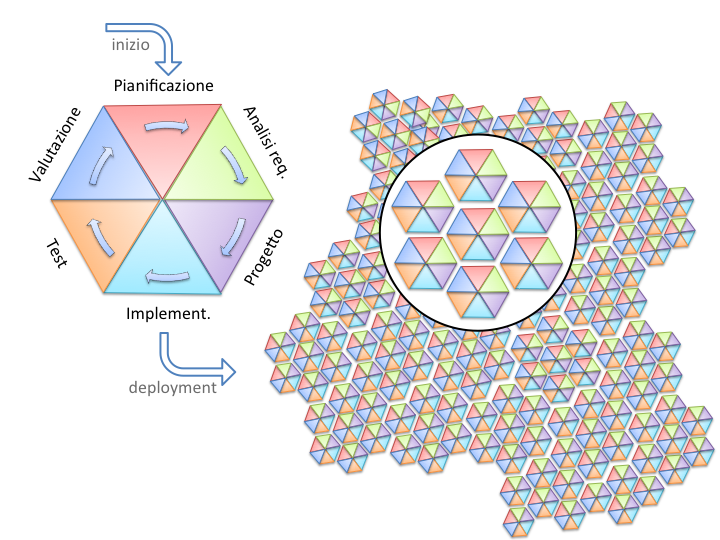
\includegraphics[scale=0.5]{img/modello_incrementale.png}
		\caption{Rappresentazione del modello incrementale\protect\footnotemark}
		\label{fig:modello_incrementale}
	\end{figure}

	\footnotetext{Fonte in \S\ref{rifinfo}}
	
\section{Descrizione generale}
testo

	\subsection{Intento del prodotto}
	testo
	
	\subsection{Funzioni del prodotto}
	testo

	\subsection{Caratteristiche degli utenti}
	testo
	
	\subsection{Vincoli del progetto}
		testo
	
		\subsubsection{Requisiti minimi}
		testo
	
		\subsubsection{Requisiti desiderabili}
		testo
%\newpage
\section{Tecnologie e scelte relative al progetto}
	L'obiettivo di questo paragrafo è descrivere in maniera specifica come \progetto\ andrà a interfacciarsi con le tecnologie.\\
	Per ciascuna di queste è previsto un \gloss{microservizio}, il quale avrà come scopo quello di fare da tramite tra lo strumento che genera il messaggio e quello che lo riceve.\\
	Questo pattern si chiama \gloss{Publisher / Subscriber} e utilizza uno strumento intermedio detto Broker per lo smistamento dei messaggi e la gestione dei flussi.

	\begin{figure}[H]
		\centering
		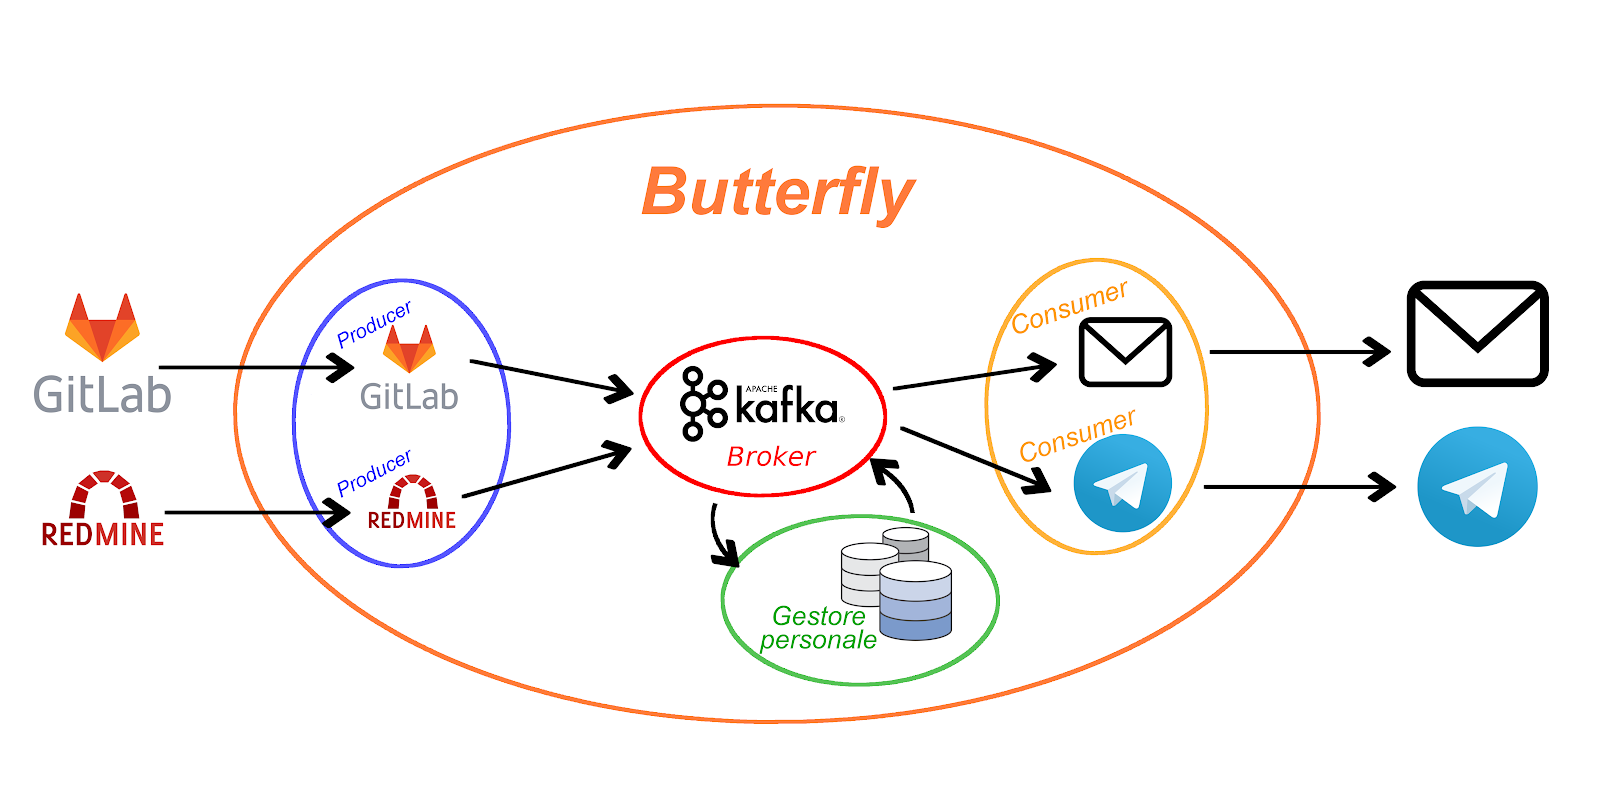
\includegraphics[width=\textwidth]{img/butterfly.png}\\
		\caption{Visione generale del sistema \progetto}
		\label{fig:butterfly}
	\end{figure}
	L'immagine precedente rappresenta una suddivisione del sistema in quattro sezioni principali:
	\begin{itemize}
		\item \progetto\ (arancione)
		\item Producer (azzurro)
		\item Broker (rosso)
		\item Consumer (verde)
	\end{itemize}
	Questa scomposizione permette di analizzare più approfonditamente i vari sottosistemi del prodotto in rapporto alle tecnologie esterne a Butterfly (GitLab, Redmine, Telegram ed e-mail), ai microservizi interni come i Producer / Consumer associati e il Broker.
	
	\subsection{Producer}
	
		Per ciascuno degli strumenti che invia messaggi verso il sistema è necessario creare una componente applicativa di tipo Producer che li riceva e li elabori inoltrandoli successivamente verso il Broker.
		Le tecnologie dalle quali vengono ricevuti i messaggi sono elencate di seguito in ordine di priorità in base a quanto richiesto dal \gloss{committente}.
		\begin{itemize}
			\item Redmine
			\item GitLab
			\item SonarQube
		\end{itemize}
		\gruppo\ ha scelto di sviluppare i Producer per le prime due applicazioni in base alle priorità suggerite da \II\ nel capitolato, lasciando l'applicativo relativo a SonarQube come opzionale.
		
		Ciascun messaggio ricevuto da queste tecnologie verrà analizzato dal Producer associato che ne ricercherà al suo interno keyword che ne indicano il Topic.
		Queste sono preimpostate da una persona incaricata dall'azienda che le inserisce nel database.
		
		\subsubsection{Redmine}
		Ciascuna istanza di Redmine permette l'utilizzo di webhook\footnote{Riferirsi alla voce ``Webhook di Redmine'' alla sezione \S\ref{sec:RiferimentiInformativi}} che inviano segnalazioni al Producer alla modifica del progetto.
		Queste vengono ricevute dal server tramite un microservizio che resta in ascolto, aggiornando in base a quello che riceve i dati presenti sul gestore personale e inoltrando le notifiche ai Consumer interessati.
		In particolare, le modifiche relative al progetto prese in considerazione sono:
		\begin{itemize}
			\item Apertura issue
		\end{itemize} 
		
		\subsubsection{GitLab}
		Ciascuna istanza di GitLab, online o in un server locale interno dell'azienda, mette a disposizione la configurazione di webhook\footnote{Riferirsi alla voce ``Webhook di GitLab'' alla sezione \S\ref{sec:RiferimentiInformativi}} che, alla modifica della \gloss{repository}, manda un messaggio con le informazioni dei cambiamenti, inseriti nella repository, a un microservizio capace di aggiornare i dati presenti nel gestore personale e, come per Redmine, inoltrare le notifiche ai Consumer interessati.
		In particolare, le modifiche relative alla repository prese in considerazione sono:
		\begin{itemize}
			\item Commit
			\item Apertura \gloss{issue}
			\item Chiusura issue
		\end{itemize}
		Le segnalazioni sono generate da commit contenenti \gloss{keyword} preimpostate.
		
%		\subsubsection{SonarQube}
%		Come GitLab, anche SonarQube prevede l'utilizzo di Webhooks\footnote{\url{https://docs.sonarqube.org/latest/project-administration/Webhooks/}} che dopo ciascuna build comunica il risultato e le informazioni relative ad essa ad un microservizio capace di aggiornare i dati presenti nel gestore personale e, anche in questo caso, inoltrare le notifiche ai customer interessati.
		
	\subsection{Broker}
	
		Il ruolo del Broker è quello smistare i messaggi in base ai Topic con cui questi sono contrassegnati verso i vari microservizi con cui l'utente ha deciso che gli venga inoltrata la notifica.
		L'azienda consiglia di utilizzare come Broker per i messaggi \gloss{Apache Kafka}.
	
		\subsubsection{Apache Kafka}
		\gloss{Apache Kafka} è un software \gloss{open source} che permette la lettura e la scrittura di messaggi su stream di dati.
		Questi messaggi arrivano dai microservizi Producer che ricevono le notifiche di applicazioni di terze parti e mandandole verso il Broker. Questo le elabora analizzandone il contenuto e contrassegnandole con Topic che verranno utilizzati per l'inoltro ai Consumer e successivamente agli utenti finali, i quali possono abbonarsi a più Topic e gestendo le proprie preferenze.		
	
	\subsection{Consumer}
		Come per gli strumenti precedentemente elencati, anche per quelli su cui il messaggio andrà ad essere inoltrato, è necessaria la creazione di un microservizio in grado di fare da tramite tra Broker e \gloss{client} dello strumento.
		Le tecnologie alle quali vengono inoltrati i messaggi sono elencate di seguito in ordine di priorità in base a quanto richiesto dal committente.
			
		\subsubsection{Telegram}
		Telegram permette l'interazione in maniera automatica con gli utenti tramite \gloss{bot} che possono essere configurati per mandare messaggi ricevuti da strumenti di terze parti.
		Il Broker manda i messaggi ad un microservizio che si occupa della trasmissione effettiva al bot di Telegram.
		%https://core.telegram.org/bots
		
		\subsubsection{E-mail}
		Per inoltrare le e-mail agli utenti finali è necessario un microservizio che sfrutta un server di posta in modo tale da poter ricevere i messaggi dal Broker e poi mandarli all'indirizzo specificato.
		%https://realpython.com/python-send-email/
		
%		\subsubsection{Slack}
%		È possibile utilizzare le API di Slack per poter mandare push notifications ai canali o alle persone interessate specificando il nome del canale (o lo username della persona), testo del messaggio, e lo username che verrà mostrato per il mittente.
%		%https://www.confluent.io/blog/real-time-syslog-processing-with-apache-kafka-and-ksql-part-2-event-driven-alerting-with-slack/
	
	\subsection{Gestore personale}
	Il gestore personale è quel \gloss{componente} che permette agli utenti di impostare le proprie preferenze per il canale di inoltro dei messaggi ed i Topic a cui ci si iscrive, interfacciandosi dunque con l'intero sistema.
	È previsto come un'applicazione web installata in un server interno all'azienda accessibile dai dipendenti interessati, i quali potranno quindi modificare, perciò con la possibilità di aggiungere e rimuovere, impostazioni come Topic a cui si è iscritti e modalità di ricezione dei messaggi.
	
	\subsection{Container Software}
	
		Un container software simula questo ambiente virtuale dove è possibile testare e mantenere le proprie applicazioni, permettendo di aumentare l'efficienza riducendone i costi e simulando l'esecuzione di sistema operativo su una macchina con \gloss{risorse} condivise.
		
		\subsection{Differenza tra container e macchina virtuale}
		A differenza delle \gloss{macchine virtuali}, dove lo stato dell'ambiente viene salvato su disco occupando memoria, i container si adattano in maniera più performante all'applicativo richiesto, in quanto il loro scopo è quello di massimizzare la quantità delle applicazioni in esecuzione riducendo al minimo il numero delle macchine per eseguirla.
		Sono quindi più leggeri, occupando meno memoria su disco e impiegando meno risorse. Purtroppo al termine della loro esecuzione non viene salvato lo stato, a meno che non sia esplicitamente richiesto.
		
		\subsubsection{Docker e Dockerfile}
		L'azienda consiglia di utilizzare \gloss{Docker} per la semplicità e perché si adatta all'architettura a microservizi.
		La configurazione avverrà tramite un \gloss{dockerfile} in cui verranno specificate informazioni come sistema operativo, script di avvio, numero di istanze ed altri parametri specifici.

	\subsection{Utenti}
		\subsubsection{Amministratore}
		\subsubsection{Utente finale}
		
	\subsection{Topic}
\newpage
\section{Casi d'uso}
testo

	\subsection{Introduzione}
	testo
	
	\subsection{Attori}
	\begin{itemize}
		\item Producer
		\item Utente che interagisce con il gestore personale
		\item Consumer (secondario)
	\end{itemize}
	
	\subsection{Elenco casi d'uso}

%TODO: da ricordarsi: se qualcuno è offline, c'è la possibilità che il messaggio venga perso.

\newcounter{uccount}

\stepcounter{uccount}
\subsubsection{UC\theuccount\ - Redmine/GitLab genera una segnalazione}
    \begin{figure}[H]
		\centering
		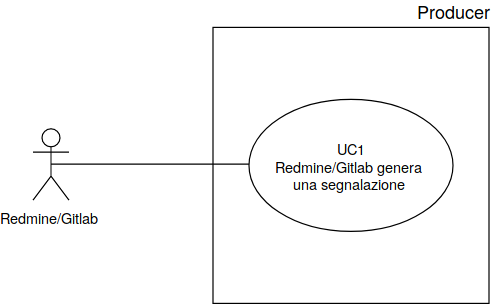
\includegraphics[width=0.7\textwidth]{img/UC1.png}\\
		\caption{UC\theuccount - Redmine/GitLab genera una segnalazione}
	\end{figure}
	\begin{itemize}
		\item \textbf{Codice}: UC\theuccount.
		\item \textbf{Titolo}: Redmine/GitLab genera una segnalazione.
		\item \textbf{Attori primari}: Redmine/Gitlab.
		\item \textbf{Descrizione}:
		 il sistema qui è il Producer ed è interno al sistema Butterfly. Cambio stato repository tramite commit per GitLab. Cambio di stato issue tracking system per GitLab e Redmine.
		\item \textbf{Precondizione}: c'è qualcosa da segnalare
		\item \textbf{Postcondizione}: segnalazione generata e inviata
		\item \textbf{Scenario principale}: 
		\begin{enumerate}
			\item Redmine/GitLab prepara una segnalazione da mandare
			\item Redmine/GitLab invia la segnalazione al Producer.
		\end{enumerate}
		
	\end{itemize}

\subsubsection{UC\theuccount.1 - Redmine/GitLab crea e invia un messaggio per il Producer}
    \begin{figure}[H]
		\centering
		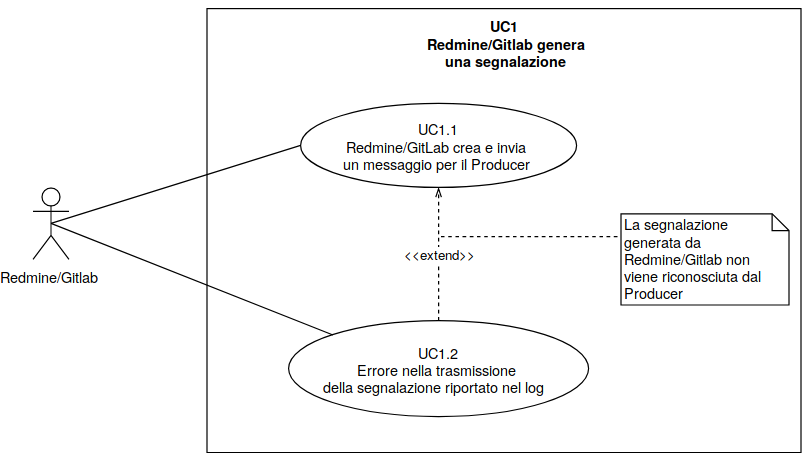
\includegraphics[width=1\textwidth]{img/UC1_1.png}\\
		\caption{UC\theuccount.1, UC\theuccount.2 - segnalazione corretta ed errata}
	\end{figure}
	\begin{itemize}
		\item \textbf{Codice}: UC\theuccount.1.
		\item \textbf{Titolo}: Redmine/GitLab crea e invia un messaggio per il Producer.
		\item \textbf{Attori primari}: Redmine/Gitlab.
		\item \textbf{Descrizione}:
		il sistema qui è il Producer ed è interno al sistema Butterfly. Cambio stato repository tramite commit per GitLab. Cambio di stato issue tracking system per GitLab e Redmine.
		\item \textbf{Precondizione}: Redmine/Gitlab generano un messaggio per il Producer
		\item \textbf{Postcondizione}: segnalazione generata e inviata al Producer
		\item \textbf{Scenario principale}: 
		\begin{enumerate}
			\item Redmine/GitLab prepara una segnalazione da mandare
			\item Redmine/GitLab invia la segnalazione al Producer.
		\end{enumerate}
		\item \textbf{Estensioni}: messaggio creato con parametri errati.
	\end{itemize}


%\subsubsection{UC\theuccount.2 - Redmine/GitLab genera una segnalazione errata}
\subsubsection{UC\theuccount.2 - Errore nella trasmissione della segnalazione}
	\begin{itemize}
		\item \textbf{Codice}: UC\theuccount.2.
		\item \textbf{Titolo}: Errore nella trasmissione della segnalazione.
		\item \textbf{Attori primari}: Redmine/Gitlab.
		\item \textbf{Descrizione}: il sistema qui è il Producer ed è interno al sistema Butterfly. Il messaggio creato da Redmine/Gitlab è errato.
		\item \textbf{Precondizione}: l'errore nella trasmissione porta alla generazione di una stringa malformata.
		\item \textbf{Postcondizione}: creazione di un log contenente informazioni utili relativi all'errore
		\item \textbf{Scenario principale}:
		\begin{enumerate}
			\item Redmine/GitLab invia una segnalazione malformata al Producer.
			\item Il producer registra l'errore nel log.
		\end{enumerate}
	\end{itemize}

\stepcounter{uccount}
\subsubsection{UC\theuccount\ - Il Producer invia una segnalazione al Broker}
	\begin{figure}[H]
		\centering
		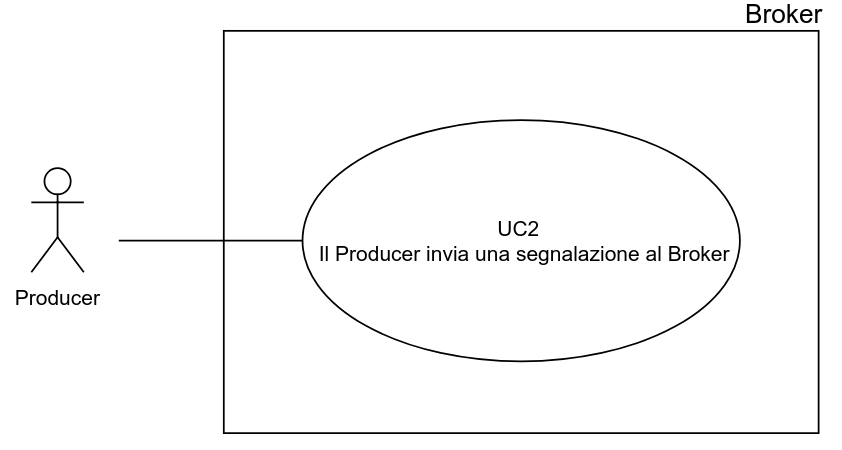
\includegraphics[width=0.7\textwidth]{img/UC2Producer.png}\\
		\caption{UC\theuccount - Il Producer invia una segnalazione al Broker}
	\end{figure}
	\begin{itemize}
		\item \textbf{Codice}: UC\theuccount.
		\item \textbf{Titolo}: il Producer invia una segnalazione al Broker.
		\item \textbf{Attori primari}: Producer.
		\item \textbf{Descrizione}: il Producer, dopo aver ricevuto una determinata segnalazione da Redmine/Gitlab, la inoltra al Broker in modo che possa istanziarne un Topic. Il sistema di riferimento qui è il Broker ed è interno al sistema Butterfly.
		\item \textbf{Precondizione}: il Producer ha ricevuto una segnalazione da inoltrare.
		\item \textbf{Postcondizione}: il Producer ha inviato al Broker la segnalazione.
		\item \textbf{Scenario principale}:
		\begin{enumerate}
			\item Il Producer procede all'invio della segnalazione
		\end{enumerate}
		 
	\end{itemize}

%Opzionale Sonarqube

\stepcounter{uccount}
\subsubsection{UC\theuccount\ - Il Consumer interroga il Broker}
	\begin{figure}[H]
		\centering
		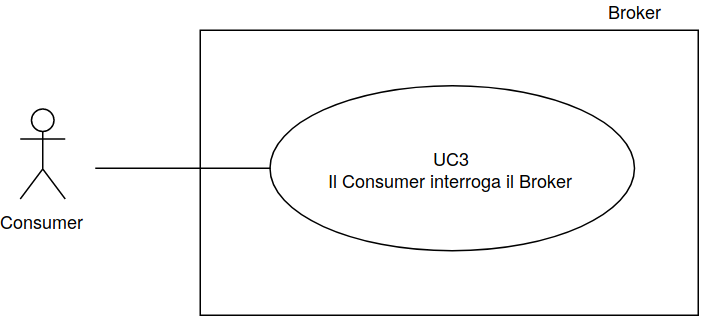
\includegraphics[width=\columnwidth]{img/UC3.png}\\
		\caption{UC\theuccount\ - Accesso}
	\end{figure}
	\begin{itemize}
		\item \textbf{Codice}: UC\theuccount.

		\item \textbf{Titolo}: il Consumer interroga il Broker.
		\item \textbf{Attori primari}: Consumer.
		\item \textbf{Descrizione}: il Consumer chiede al Broker di acquisire il messaggio da inoltrare verso il client della tecnologia specificata dall'utente finale. Il sistema di riferimento qui è Broker ed è interno al sistema Butterfly.
		\item \textbf{Precondizione}: il Broker ha un messaggio pronto ad essere inoltrato da un Consumer verso un client delle tecnologie con cui il sistema si interfaccia.
		\item \textbf{Postcondizione}: dopo aver recuperato il messaggio dal Broker il Consumer lo inoltra al client della tecnologia correlata in attesa con lo scopo l'utente finale lo legga.
		\item \textbf{Scenario principale}: 
			\begin{enumerate}
				\item Il Consumer richiede la segnalazione da inviare al client utilizzato dall'utente finale
			\end{enumerate}
	\end{itemize}

\stepcounter{uccount}
\subsubsection{UC\theuccount\ - Telegram/mail riceve un messaggio dal Consumer}
	\begin{figure}[H]
		\centering
			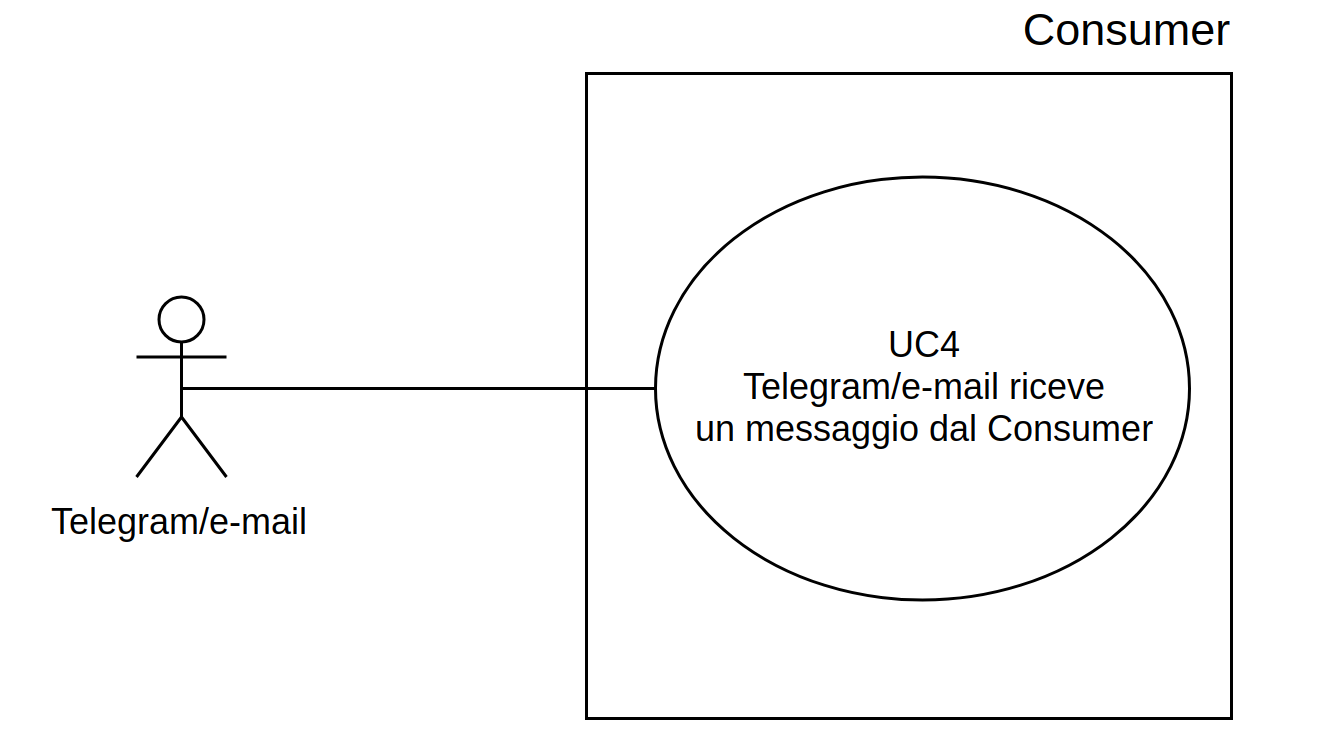
\includegraphics[width=\columnwidth]{img/UC4.png}\\
		\caption{UC\theuccount\ - Telegram/mail riceve un messaggio dal Consumer}
	\end{figure}
	\begin{itemize}
		\item \textbf{Codice}: UC\theuccount.
		\item \textbf{Titolo}: Telegram/mail riceve un messaggio dal Consumer.
		\item \textbf{Attori}: Telegram/server mail.
		\item \textbf{Descrizione}: il sistema di riferimento qui è il Consumer ed è interno al sistema Butterfly.
		Sebbene questo caso d'uso non sia del tutto corretto perchè l'attore Telegram/mail è un attore passivo, che riceve e non che agisce, è stato scelto di creare questo caso d'uso al fine di inserire la funzionalità "Il Consumer invia un messaggio a Telegram/mail". Ma scrivere un caso d'uso in tal modo sarebbe stato del tutto scorretto in quanto il sistema di riferimento in questo caso sarebbe stato Telegram/mail. Cosa non possibile dato che Telegram/mail è esterno a Butterfly e quindi non può essere considerato un suo sottosistema.
		\item \textbf{Precondizione}: il Consumer invia un messaggio a Telegram/server email in seguito a un'interrogazione del broker.
		\item \textbf{Postcondizione}: Telegram/server mail riceve il messaggio
		\item \textbf{Scenario principale}:
		\begin{enumerate}
			\item La ricezione del messaggio va a buon fine
		\end{enumerate} 
	\end{itemize}

% Opzionale Slack

\stepcounter{uccount}
\subsubsection{UC\theuccount\ - Accesso}
		\begin{figure}[H]
			\centering
				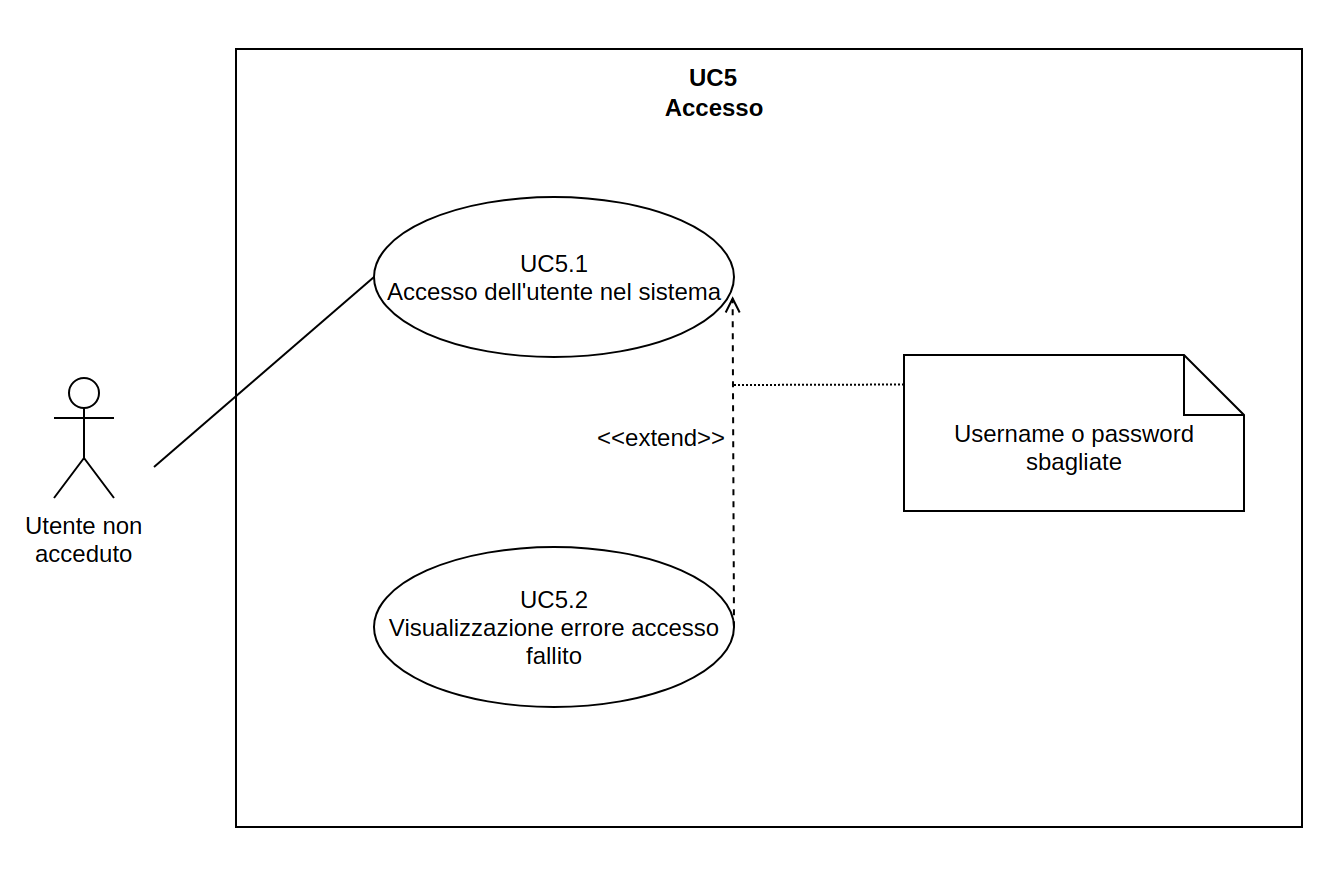
\includegraphics[width=\columnwidth]{img/UC5.png}\\
			\caption{UC\theuccount\ - Accesso}
		\end{figure}
	\begin{itemize}
		\item \textbf{Codice}: UC5
		\item \textbf{Titolo}: accesso
		\item \textbf{Attori primari}: utente non acceduto
		\item \textbf{Descrizione}: l'utente richiede di accedere al sistema attraverso un form dove inserisce username e password
		\item \textbf{Precondizione}: il sistema considera l’utilizzatore come un utente non acceduto
		\item \textbf{Postcondizione}: il sistema riconosce l'utilizzatore come utente acceduto
		\item \textbf{Scenario Principale}: l'utente non ancora riconosciuto dal sistema effettua l'accesso.
	\end{itemize}
	
	\paragraph{UC\theuccount.1 - Accesso dell'utente nel sistema}
		\begin{figure}[H]
			\centering
				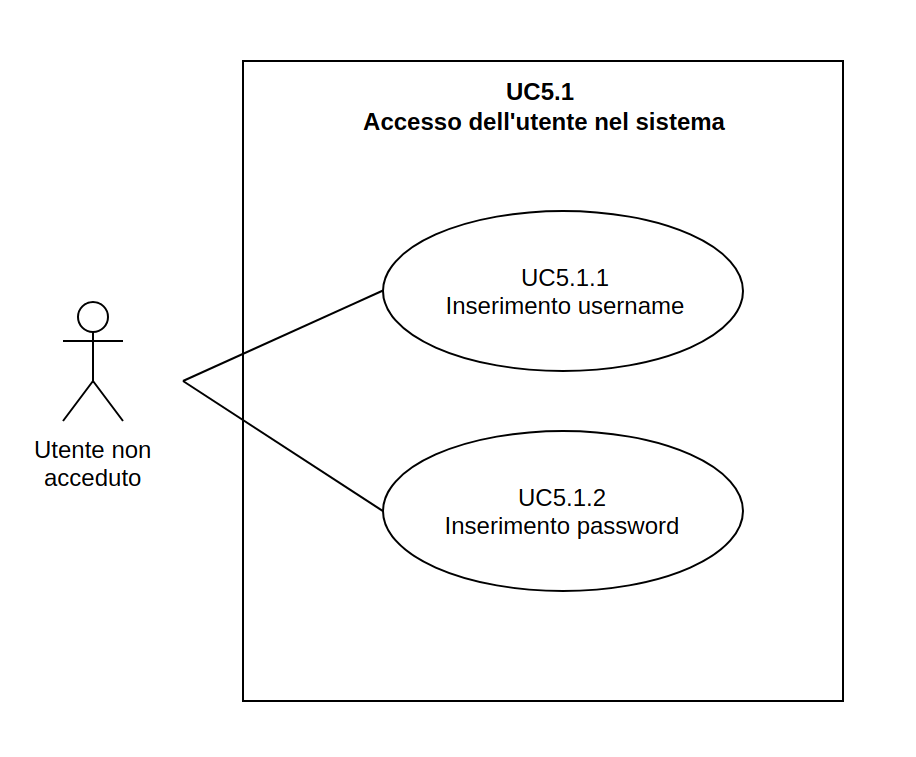
\includegraphics[width=\columnwidth]{img/UC5_1.png}\\
			\caption{UC\theuccount.1 - Accesso dell'utente nel sistema}
		\end{figure}
		\begin{itemize}
			\item \textbf{Codice}: UC\theuccount.1
			\item \textbf{Titolo}: accesso dell'utente nel sistema
			\item \textbf{Attori}: utente non acceduto
			\item \textbf{Descrizione}: l'utente attende l'autenticazione da parte del sistema
			\item \textbf{Precondizione}: il sistema riconosce l'utilizzatore come un utente non autenticato
			\item \textbf{Postcondizione}: il sistema riconosce l'utente autenticato con successo
			\item \textbf{Scenario Principale}: l’utente non ancora riconosciuto dal sistema richiede l'autenticazione
			\item \textbf{Estensioni}:
			\begin{enumerate}
				\item Nel caso in cui l'accesso non dovrebbe andare a buon fine viene visualizzato un errore avvisando l'utente [UC5.2].
			\end{enumerate}
	\end{itemize}

		\subparagraph{UC\theuccount.1.1 - Inserimento username}
			\begin{itemize}
				\item \textbf{Codice}: UC\theuccount.1.1
				\item \textbf{Titolo}: inserimento username
				\item \textbf{Attori}: utente non acceduto
				\item \textbf{Descrizione}: l'utente inserisce l'username
				\item \textbf{Precondizione}: il sistema offre l'interfaccia grafica adatta all'inserimento dell'username
				\item \textbf{Postcondizione}: l'utente ha inserito l'username desiderato
				\item \textbf{Scenario Principale}: l'utente inserisce l'username per autenticarsi.
			\end{itemize}
		
		\subparagraph{UC\theuccount.1.2 - Inserimento password}
			\begin{itemize}
				\item \textbf{Codice}: UC\theuccount.1.2	
				\item \textbf{Titolo}: inserimento password
				\item \textbf{Attori}: utente non acceduto
				\item \textbf{Descrizione}: l'utente inserisce la password
				\item \textbf{Precondizione}: il sistema offre l'interfaccia grafica adatta all'inserimento della password
				\item \textbf{Postcondizione}: l'utente ha inserito la password desiderata
				\item \textbf{Scenario Principale}: l'utente inserisce la password per autenticarsi.
			\end{itemize}
		
%Da aggiungere al limite più avanti
		
%		\subparagraph{UC5.1.2}
%			\begin{itemize}
%			\item \textbf{Codice}: UC6.1.2.
%			\item \textbf{Titolo}: inserimento password
%			\item \textbf{Attori}: utente non autenticato
%			\item \textbf{Descrizione}: l'utente inserisce la password
%			\item \textbf{Precondizione}: il sistema offre l'interfaccia grafica adatta all'inserimento della password
%			\item \textbf{Postcondizione}: l'utente ha inserito la password desiderata
%			\item \textbf{Scenario Principale}: l'utente inserisce la password per autenticarsi
%		\end{itemize}
	
	\paragraph{UC\theuccount.2 - Visualizzazione errore autenticazione fallita}
		\begin{itemize}
			\item \textbf{Titolo}: visualizzazione errore autenticazione fallita
			\item \textbf{Attori}: utente non autenticato
			\item \textbf{Descrizione}: l'utente viene avvisato che ha inserito username o password errate
			\item \textbf{Precondizione}: il sistema riceve una richiesta di accesso da parte di un utente che
			fornisce username o password sbagliate
			\item \textbf{Postcondizione}: il sistema comunica all'utilizzatore l'errore
			\item \textbf{Scenario Principale}: l'utente visualizza il messaggio d'errore.
		\end{itemize}


\stepcounter{uccount}
\subsubsection{UC\theuccount\ - Modifica delle preferenze}
	\begin{figure}[H]
		\centering
		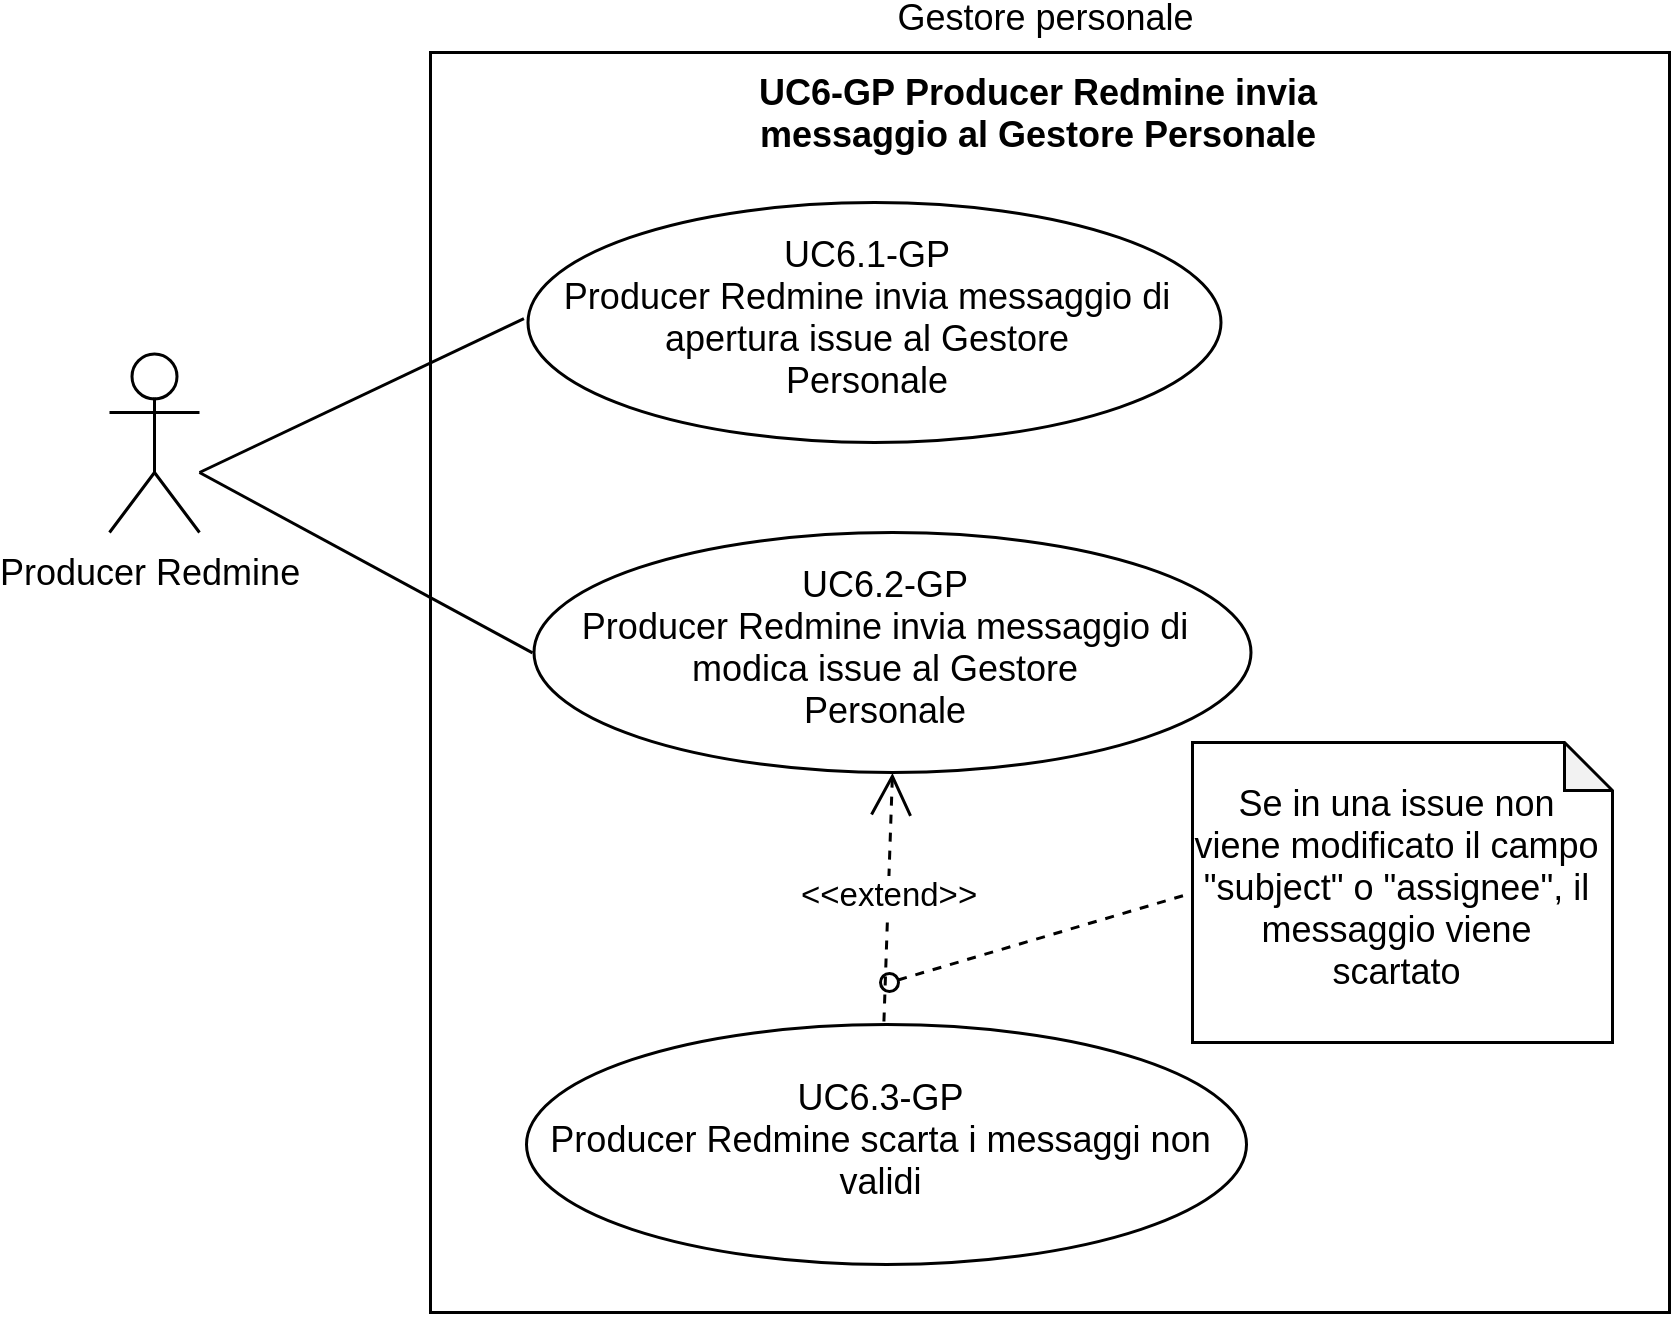
\includegraphics[width=\columnwidth]{img/UC6.png}\\
		\caption{UC\theuccount\ - Modifica delle preferenze}
	\end{figure}
	\begin{itemize}
		\item \textbf{Codice}: UC\theuccount.
		\item \textbf{Titolo}: modifica delle preferenze.
		\item \textbf{Attori}: Utente.
		\item \textbf{Descrizione}: attraverso un'interfaccia l'utente può modificare i vari parametri per configurare l'applicazione per le proprie esigenze. Il sistema di riferimento considerato è tutto \progetto.
		\item \textbf{Precondizione}: l'utente ha acceduto con le sue credenziali corrette nel sistema.
		\item \textbf{Postcondizione}: l'utente effettua zero o più modifiche nella configurazione personale dell'applicazione. 
		\item \textbf{Scenario Principale}: L'utente ha la possibilità di portare delle modifiche alle sue preferenze all'interno dell'applicazione \progetto.
	\end{itemize}



	\paragraph{UC\theuccount.1 - Aggiunta preferenze}
		\begin{figure}[H]
			\centering
			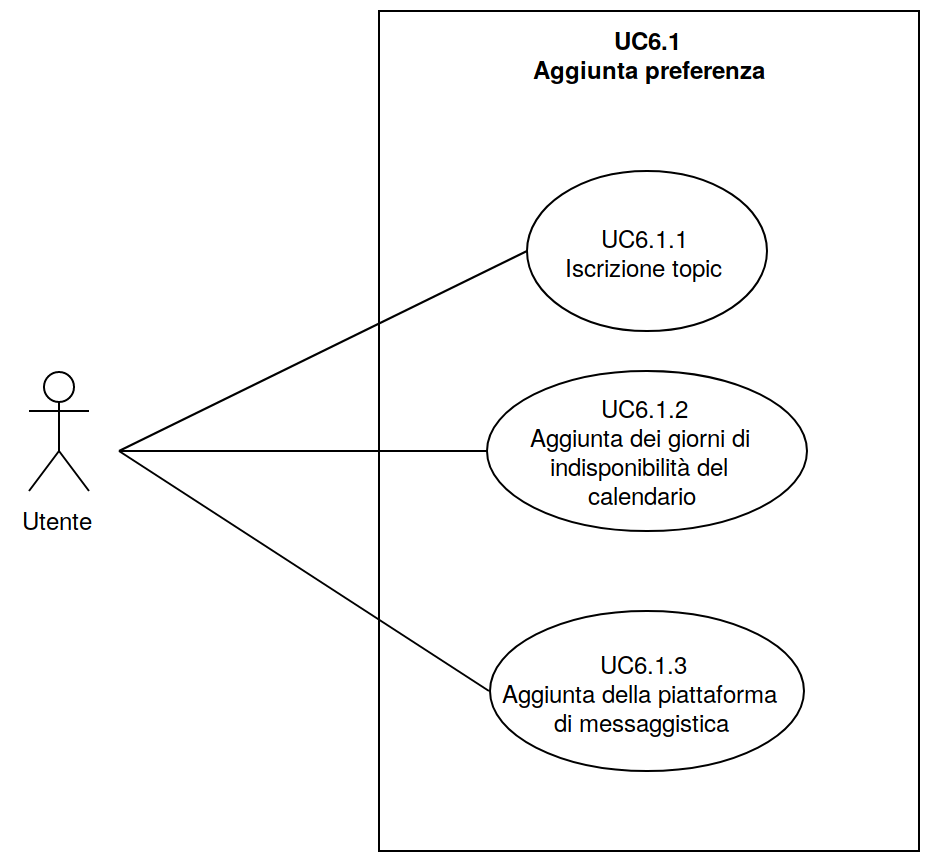
\includegraphics[width=\columnwidth]{img/UC6_1.png}\\
			\caption{UC\theuccount.1 - Aggiunta preferenze}
		\end{figure}
	\begin{itemize}
		\item \textbf{Codice}: UC\theuccount.1.
		\item \textbf{Titolo}: aggiunta preferenze.
		\item \textbf{Descrizione}: l'utente, date le varie opzioni per configurare \progetto, aggiunge una preferenza tra topic, giorni di calendario e piattaforme di messaggistica.
		\item \textbf{Precondizione}: l'utente ha acceduto con le sue credenziali corrette nel sistema e non ha selezionato tutte le preferenze possibili proposte da \progetto.
		\item \textbf{Postcondizione}: lo nuova configurazione contiene una o più preferenza in aggiunta rispetto alla quella precedente.
		\item \textbf{Scenario principale}: l'utente può scegliere, tra le varie opzioni disponibili disponi, quale aggiungere alla sua configurazione personale.
	\end{itemize}
	
	\subparagraph{UC\theuccount.1.1 - Iscrizione topic}
	\begin{itemize}
		\item \textbf{Codice}: UC\theuccount.1.1.
		\item \textbf{Titolo}: iscrizione topic.
		\item \textbf{Descrizione}: data la lista di topic presenti già inserita precedentemente, l'utente seleziona quelli a cui è interessato volendone ricevere una notifica. I topic sono divisi per categoria comprendendo etichette o parole chiave stabilite in precedenza.
		\item \textbf{Precondizione}: l'utente ha acceduto con le sue credenziali corrette nel sistema e non ha selezionato tutte le preferenze possibili proposte da \progetto.
		\item \textbf{Postcondizione}: il numero di topic a cui è interessato l'utente è aumentato.
		\item \textbf{Scenario principale}: l'utente aggiunge un topic dalla lista proposta dall'applicazione \progetto.
	\end{itemize}
		
			
	\subparagraph{UC\theuccount.1.2 - Aggiunta giorno irreperibilità nel calendario} 
	\begin{itemize}
		\item \textbf{Codice}: UC\theuccount.1.2.
		\item \textbf{Titolo}: aggiunta dei giorni di indisponibilità nel calendario.
		\item \textbf{Descrizione}: dato il calendario lavorativo, l'utente aggiunge i giorni in cui è reperibile e non vuole ricevere notifiche.
		\item \textbf{Precondizione}: l'utente ha acceduto con le sue credenziali corrette nel sistema e non ha selezionato tutte le preferenze possibili proposte da \progetto.
		\item \textbf{Postcondizione}: il numero di giorni in cui l'utente non si rende disponibile.
		\item \textbf{Scenario principale}: l'utente aggiunge le date di calendario in cui non è reperibile.
	\end{itemize}
			
	\subparagraph{UC\theuccount.1.3 - Aggiunta della piattaforma di messaggistica}
	\begin{itemize}
		\item \textbf{Codice}: UC\theuccount.1.3.
		\item \textbf{Titolo}:aggiunta della piattaforma di messaggistica.
		\item \textbf{Descrizione}: dalla lista delle piattaforme di messaggistica l'utente aggiunge quelle da cui vuole ricevere le notifiche.
		\item \textbf{Precondizione}: l'utente ha acceduto con le sue credenziali corrette nel sistema e non ha selezionato tutte le preferenze possibili proposte da \progetto.
		\item \textbf{Postcondizione}: il numero di piattaforme di messaggistica selezionate dall'utente è aumentato.
		\item \textbf{Scenario principale}: l'utente aggiunge le piattaforme di messaggistica da un elenco già fornito. 
		%telegram: nickname e mail sono già salvati nel DB
	\end{itemize}
			



	\paragraph{UC\theuccount.2 - Rimozione preferenza}
		\begin{figure}[H]
			\centering
			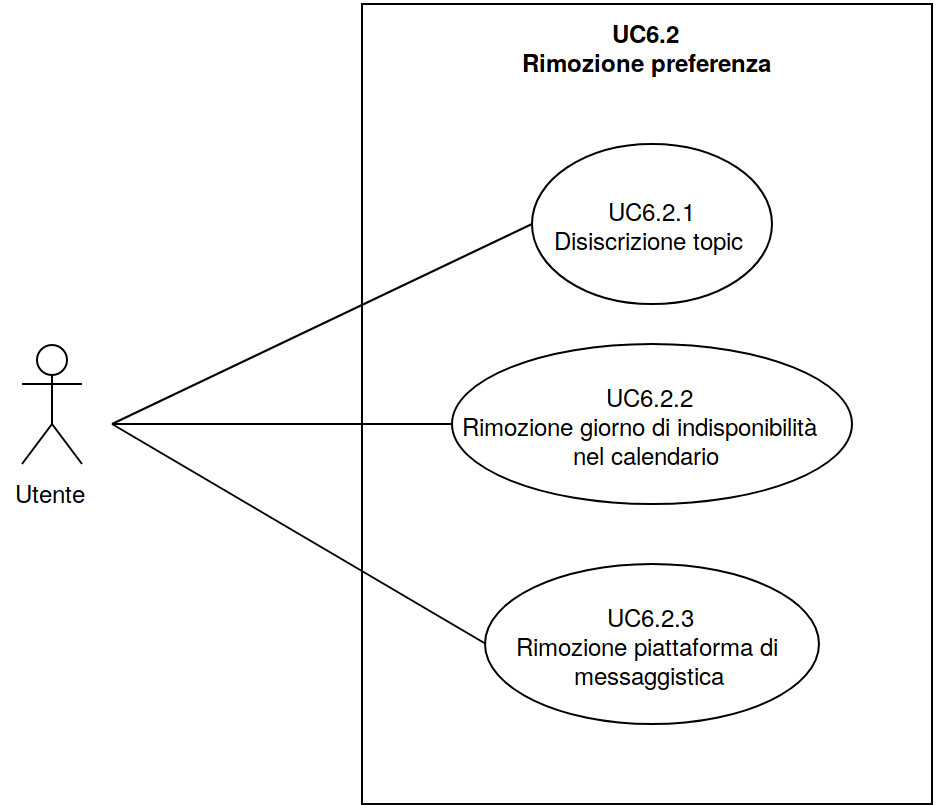
\includegraphics[width=\columnwidth]{img/UC6_2.png}\\
			\caption{UC\theuccount.2 - Rimozione preferenza}
		\end{figure}
	\begin{itemize}
		\item \textbf{Codice}: UC\theuccount.2.
		\item \textbf{Titolo}: rimozione preferenza.
		\item \textbf{Descrizione}: l'utente, dopo aver selezionato delle preferenze dalle opzioni di configurazione, ne rimuove una o di più. Le preferenze consistono in topic, date di calendario e piattaforme di messaggistica.
		\item \textbf{Precondizione}: l'utente ha acceduto con le credenziali nel sistema ed è presente almeno una preferenza selezionata tra quelle proposte da \progetto.
		\item \textbf{Postcondizione}: la nuova configurazione contiene una o più configurazioni in meno rispetto a quella precedente.
		\item \textbf{Scenario principale}: l'utente selezione tra le preferenze già scelte precedentemente quale rimuovere.
	\end{itemize}
	
	
	\subparagraph{UC\theuccount.2.1 - Disiscrizione topic}
	\begin{itemize}
		\item \textbf{Codice}: UC\theuccount.2.1.
		\item \textbf{Titolo}: disiscrizione topic.
		\item \textbf{Descrizione}: l'utente di disiscrive da un topic da uno o o più topic dai quali prima riceveva delle notifiche.
		\item \textbf{Precondizione}: l'utente ha acceduto con le credenziali nel sistema ed è presente almeno una preferenza selezionata tra quelle proposte da \progetto.
		\item \textbf{Postcondizione}: il numero di topic a cui è iscritto un utente è diminuito.
		\item \textbf{Scenario principale}: l'utente seleziona i topic a cui si era iscritto precedentemente per disicriversi.
	\end{itemize}
	
			
	\subparagraph{UC\theuccount.2.2 - Rimozione giorno irreperibilità nel calendario}
	\begin{itemize}
		\item \textbf{Codice}: UC\theuccount.2.2.
		\item \textbf{Titolo}: rimozione giorno irreperibilità nel calendario.
		\item \textbf{Descrizione}: l'utente rimuove i giorni di calendario in cui precedentemente non era reperibile.
		\item \textbf{Precondizione}: l'utente ha acceduto con le credenziali nel sistema ed è presente almeno una preferenza selezionata tra quelle proposte da \progetto.
		\item \textbf{Postcondizione}: il numero di giorni di calendario in cui l'utente non è reperibile è diminuito.
		\item \textbf{Scenario principale}: l'utente, dopo aver visto i giorni in cui si era segnato non reperibile, ne rimuove alcuni rendendosi disponibile in quelle date.
	\end{itemize}
			
			
	\subparagraph{UC\theuccount.2.3 - Rimozione piattaforma di messaggistica}
	\begin{itemize}
		\item \textbf{Codice}: UC\theuccount.2.3.
		\item \textbf{Titolo}: rimozione piattaforma di messaggistica.
		\item \textbf{Descrizione}: l'utente rimuove le piattaforme di messaggistica dalle quali non vuole più ricevere notifiche tramite \progetto.
		\item \textbf{Precondizione}: l'utente ha acceduto con le credenziali nel sistema ed è presente almeno una preferenza selezionata tra quelle proposte da \progetto.
		\item \textbf{Postcondizione}: il numero di piattaforme di messaggistica da cui l'utente vuole ricevere notifiche è diminuito.
		\item \textbf{Scenario principale}: l'utente seleziona da un elenco già presente le piattaforme di messaggistica che aveva precedentemente selezionato da cui non vuole più ricevere notifiche tramite \progetto.
	\end{itemize}

%Da tenere in considerazione per la pagina da creare più avanti	
%	\paragraph{UC7.4}
%	Annullo le modifiche fatte

		

\newpage
\section{Requisiti}
Ad ogni requisito viene assegnato il codice identificativo univoco:
	\begin{center}
		\texttt{R[Numero][Tipo][Priorità]}
	\end{center}
	in cui ogni parte ha un significato preciso:
	\begin{itemize}
		\item \textbf{R}: requisito.
		\item \textbf{Numero}: numero progressivo che segue la struttura dei documenti.
		\item \textbf{Tipo}: la la tipologia di requisito che può essere di:
		\begin{itemize}
			\item \textbf{F}: funzionalità.
			\item \textbf{Q}: \gloss{qualità}.
			\item \textbf{V}: vincolo.
		\end{itemize}
		\item \textbf{Priorità}: indica il grado di urgenza di un requisito di essere soddisfatto, come:
		\begin{itemize}
			\item \textbf{0}: opzionale.
			\item \textbf{1}: desiderabile.
			\item \textbf{2}: obbligatorio.
		\end{itemize}
	\end{itemize}


	Esempio: \texttt{R2Q1} indica il secondo requisito di qualità ed è desiderabile.

	%I requisiti di seguito riportati sono elencati in modo tale da seguire la struttura dei documenti. Ovvero, si possono trovare raggruppati i requisiti derivanti dello stesso tipo, ad esempio solo i requisiti di funzionalità dal sesto al diciannovesimo derivano dai casi d'uso.
	%TODO: rifare id requisiti

%inserire il fatto che una persona può aggiungere il proprio nickname o altro da interfaccia, come requisito opzionale	...

% Generazione automatica dei numeri
%\newcounter{vaZ} % valore
%\newcommand{\incrZ}{\addtocounter{vaZ}{+1}} % Comando per l'aumento automatico del counter vaZ
%\newcommand{\addZNumber}[0]{\incrZ\thevaZ} % Comando per generare
%
%\newcommand{\Freq}[3]{R\addZNumber F#1 & #2 & #3 \\}
%\newcommand{\Fsubreq}[3]{R\thevaZ F#1 & #2 & #3 \\} % Se c'è bisogno di sottocasi

% Comando requisito generico
\newcommand{\req}[3]{%
#1 & #2 & #3 \\
}

	%COMANDI PER REQ DI FUNZIONALITÀ
	% Generazione automatica dei numeri
	\newcounter{vaF} % valore
	\newcounter{secF}[vaF] % per il secondo livello del requisito
	\newcounter{thF}[secF] % terzo livello

	\newcommand{\ReqF}[3]{\stepcounter{vaF}R\thevaF F#1 & #2 & #3 \\} % Primo livello
	\newcommand{\subReqF}[3]{\stepcounter{secF}R\thevaF.\thesecF F#1 & #2 & #3 \\} % Secondo livello
	\newcommand{\subsubReqF}[3]{\stepcounter{thF}R\thevaF.\thesecF.\thethF F#1 & #2 & #3 \\} % Terzo livello

	\newcounter{tableCounter} % Per automatizzare conteggio tabelle

	\subsection{Requisiti di funzionalità}\label{RequisitiFunzionalità}

	\stepcounter{tableCounter}
	\begin{table}[H]
		\begin{paddedtablex}[1.7]{\textwidth}{cXc}%0 opz  2 obb
			\rowcolor{white} \textbf{Codice} & \textbf{Requisito} & \textbf{Fonte} \\\toprule

			% \stepcounter{vaF} % Per allineare i requisiti ai casi d'uso

			% da casi d'uso
			\rowcolor{\tablegray}\ReqF{2}{Redmine deve poter inviare la segnalazione di apertura issue al Producer Redmine}{Interno UC1-PR}
			\rowcolor{white}\ReqF{2}{Redmine deve poter inviare la segnalazione di modifica issue al Producer Redmine}{Interno UC2-PR}
			\rowcolor{\tablegray}\ReqF{2}{GitLab deve essere in grado di segnalare l'apertura di issue al Producer GitLab}{Interno UC3-PG}
			\rowcolor{white}\ReqF{2}{GitLab deve essere in grado di segnalare la modifica issue al Producer GitLab}{Interno UC4-PG}
			\rowcolor{\tablegray}\ReqF{2}{GitLab deve poter segnalare un evento di push al Producer GitLab}{Interno UC5-PG}
			\rowcolor{white}\ReqF{2}{Il Producer Redmine deve essere in grado di inviare un messaggio al Gestore Personale}{Interno UC6-GP}
				\rowcolor{\tablegray}\subReqF{2}{Il Producer Redmine deve essere in grado di inviare un messaggio di apertura issue al Gestore Personale}{Interno UC6.1-GP}
				\rowcolor{white}\subReqF{2}{Il Producer Redmine deve essere in grado di inviare un messaggio di modifica issue al Gestore Personale}{Interno UC6.2-GP}
			\rowcolor{\tablegray}\ReqF{1}{Il Producer Redmine deve essere in grado di scartare i messaggi non validi}{Interno UC6.3-GP}
			\rowcolor{white}\ReqF{2}{Il Producer GitLab deve essere in grado di inviare un messaggio al Gestore Personale}{Interno UC7-GP}
				\rowcolor{\tablegray}\subReqF{2}{Il Producer GitLab deve essere in grado di inviare messaggi di commit al Gestore Personale}{Interno UC7.1-GP}
				\rowcolor{white}\subReqF{2}{Il Producer GitLab deve essere in grado di inviare un messaggio di issue al Gestore Personale}{Interno UC7.2-GP}
					\rowcolor{\tablegray}\subsubReqF{2}{Il Producer GitLab deve essere in grado di inviare un messaggio di nuova issue al Gestore Personale}{Interno UC7.2.1-GP}
					\rowcolor{white}\subsubReqF{2}{Il Producer GitLab deve essere in grado di inviare un messaggio di modifica issue al Gestore Personale}{Interno UC7.2.2-GP}
			\rowcolor{\tablegray}\ReqF{1}{Il Producer GitLab deve essere in grado di scartare i messaggi di issue non validi}{Interno UC7.2.3-GP}
			\rowcolor{white}\ReqF{2}{Il Gestore Personale deve poter inviare il messaggio finale al Consumer Telegram}{Interno UC8-CT}

			\bottomrule\\
		\end{paddedtablex}
		\caption{Elenco dei requisiti di funzionalità (\thetableCounter)}
	\end{table}

	\stepcounter{tableCounter}
	\begin{table}[H]
		\begin{paddedtablex}[1.7]{\textwidth}{cXc}%0 opz  2 obb
			\rowcolor{white}\textbf{Codice} & \textbf{Requisito} & \textbf{Fonte} \\\toprule

			\rowcolor{\tablegray}\ReqF{2}{Il Gestore Personale deve poter inviare il messaggio finale al Consumer Email}{Interno UC9-CE}
			\rowcolor{white}\ReqF{2}{Il Consumer Telegram deve poter inoltrare il messaggio finale al bot Telegram}{Interno UC10-BT}
			\rowcolor{\tablegray}\ReqF{2}{Il Consumer Email deve poter inoltrare il messaggio finale al server Email}{Interno UC11-SE}
			% \stepcounter{vaF} e usare \subReqF per rientrare di un livello
			\rowcolor{white}\ReqF{0}{L'utente può eseguire l'accesso al Gestore Personale}{Interno UC12.1-GP}
				\rowcolor{\tablegray}\subReqF{0}{L'utente può inserire il proprio identificativo all'interno del sistema}{Interno UC12.1.1}
			\rowcolor{white}\ReqF{0}{\progetto\ fa apparire un messaggio di errore se il tentativo di accesso non è andato a buon fine}{Interno UC12.1.2}
			\rowcolor{\tablegray}\ReqF{0}{L'utente acceduto deve poter uscire dal sistema}{Interno UC13-GP}
			\rowcolor{white}\ReqF{0}{L'utente acceduto deve poter aggiungere un nuovo utente}{Interno UC14-GP}
				\rowcolor{\tablegray}\subReqF{0}{L'utente acceduto deve poter inserire il nome dell'utente da aggiungere}{Interno UC14.1.1-GP}
				\rowcolor{white}\subReqF{0}{L'utente acceduto deve poter inserire il cognome dell'utente da aggiungere}{Interno UC14.1.2-GP}
				\rowcolor{\tablegray}\subReqF{0}{L'utente acceduto deve poter inserire il contatto Email dell'utente da aggiungere}{Interno UC14.1.3-GP}
					\rowcolor{white}\subsubReqF{0}{L'utente acceduto deve poter visualizzare un messaggio di errore se il contatto Email non è univoco}{Interno UC14.2-GP}
				\rowcolor{\tablegray}\subReqF{0}{L'utente acceduto deve poter inserire il contatto Telegram dell'utente da aggiungere}{Interno UC14.1.4-GP}
					\rowcolor{white}\subsubReqF{0}{L'utente acceduto deve poter visualizzare un messaggio di errore se il contatto Telegram non è univoco}{Interno UC14.2-GP}
			\rowcolor{\tablegray}\ReqF{0}{L'utente acceduto deve poter rimuovere un utente presente nel sistema}{Interno UC15-GP}
			% \stepcounter{secF}
				\rowcolor{white}\subReqF{0}{L'utente acceduto deve poter inserire il contatto Email dell'utente da rimuovere}{Interno UC15.1.1-GP}
				\rowcolor{\tablegray}\subReqF{0}{L'utente acceduto deve poter inserire il contatto Telegram dell'utente da rimuovere}{Interno UC15.1.2-GP}
				\rowcolor{white}\subReqF{0}{L'utente acceduto deve poter visualizzare un messaggio di errore se l'identificativo non è presente nel sistema}{Interno UC15.2-GP}

			\bottomrule
		\end{paddedtablex}
		\caption{Elenco dei requisiti di funzionalità (\thetableCounter)}
	\end{table}

	\stepcounter{tableCounter}
	\begin{table}[H]
		\begin{paddedtablex}[1.7]{\textwidth}{cXc}%0 opz  2 obb
			\rowcolor{white}\textbf{Codice} & \textbf{Requisito} & \textbf{Fonte} \\\toprule

				\rowcolor{\tablegray}\subReqF{0}{L'utente acceduto deve potersi rimuovere dal sistema}{Interno UC15.3-GP}
			\rowcolor{white}\ReqF{0}{L'utente acceduto deve poter modificare le informazioni relative a un utente}{Interno UC16-GP}
				\rowcolor{\tablegray}\subReqF{0}{L'utente acceduto deve poter selezionare l'identificativo dell'utente da modificare}{Interno UC16.1-GP}
					\rowcolor{white}\subsubReqF{0}{L'utente acceduto deve poter visualizzare un messaggio di errore se l'identificativo non è riconosciuto dal sistema}{Interno UC16.2-GP}
				\rowcolor{\tablegray}\subReqF{0}{L'utente acceduto deve poter scegliere il nuovo nome dell'utente da modificare}{Interno UC16.1.1.1-GP}
				\rowcolor{white}\subReqF{0}{L'utente acceduto deve poter scegliere il nuovo cognome dell'utente da modificare}{Interno UC16.1.1.2-GP}
				\rowcolor{\tablegray}\subReqF{0}{L'utente acceduto deve poter scegliere il nuovo contatto Email dell'utente da modificare}{Interno UC16.1.1.3-GP}
					\rowcolor{white}\subsubReqF{0}{L'utente acceduto deve poter visualizzare un messaggio di errore se il contatto Email è già presente}{Interno UC16.1.2-GP}
				\rowcolor{\tablegray}\subReqF{0}{L'utente acceduto deve poter scegliere il nuovo contatto Telegram dell'utente da modificare}{Interno UC16.1.1.4-GP}
					\rowcolor{white}\subsubReqF{0}{L'utente acceduto deve poter visualizzare un messaggio di errore se il contatto Telegram è già presente}{Interno UC16.1.2-GP}

			%\stepcounter{vaF}
			\rowcolor{\tablegray}\ReqF{0}{L'utente acceduto deve poter aggiungere le proprie preferenze nel sistema}{Interno UC17-GP}
				\rowcolor{white}\subReqF{0}{L'utente acceduto deve poter aggiungere nuovi Topic di iscrizione}{Interno UC17.1-GP}
				\rowcolor{\tablegray}\subReqF{0}{L'utente acceduto deve poter aggungere nuovi giorni di indisponibilità nel calendario}{Interno UC17.2-GP}
				\rowcolor{white}\subReqF{0}{L'utente acceduto deve poter aggungere una nuova piattaforma di messaggistica preferita}{Interno UC17.3-GP}
				\rowcolor{\tablegray}\subReqF{0}{L'utente acceduto deve poter aggungere la propria persona di fiducia}{Interno UC17.4-GP}
					\rowcolor{white}\subsubReqF{0}{L'utente acceduto deve poter visualizzare un messaggio di errore se il contatto Email della persona di fiducia non è presente nel sistema}{Interno UC17.5-GP}

			\bottomrule\\
		\end{paddedtablex}
		\caption{Elenco dei requisiti di funzionalità (\thetableCounter)}
	\end{table}

	\stepcounter{tableCounter}
	\begin{table}[H]
		\begin{paddedtablex}[1.7]{\textwidth}{cXc}%0 opz  2 obb
			\textbf{Codice} & \textbf{Requisito} & \textbf{Fonte} \\\toprule

					\subsubReqF{0}{L'utente acceduto deve poter visualizzare un messaggio di errore se il contatto Telegram della persona di fiducia non è presente nel sistema}{Interno UC17.5-GP}
				\subReqF{0}{L'utente acceduto deve poter aggiungere nuove keyword di interesse per i messaggi di commit di GitLab}{Interno UC17.6-GP}
					\subsubReqF{0}{L'utente acceduto deve poter visualizzare un messaggio di errore se la keyword inserita era già nella sua lista}{Interno UC17.7-GP}

			%\stepcounter{vaF}
			\ReqF{0}{L'utente acceduto deve poter rimuovere le proprie preferenze dal sistema}{Interno UC18-GP}
				\subReqF{0}{L'utente acceduto deve poter rimuovere i Topic a cui è iscritto}{Interno UC18.1-GP}
				\subReqF{0}{L'utente acceduto deve poter rimuovere giorni di indisponibilità nel calendario}{Interno UC18.2-GP}
				\subReqF{0}{L'utente acceduto deve poter rimuovere una piattaforma di messaggistica preferita}{Interno UC18.3-GP}
				\subReqF{0}{L'utente acceduto deve poter rimuovere la propria persona di fiducia}{Interno UC18.4-GP}
					\subsubReqF{0}{L'utente acceduto deve poter visualizzare un messaggio di errore se il contatto Email della persona di fiducia non è presente nel sistema}{Interno UC18.5-GP}
					\subsubReqF{0}{L'utente acceduto deve poter visualizzare un messaggio di errore se il contatto Telegram della persona di fiducia non è presente nel sistema}{Interno UC18.5-GP}
				\subReqF{0}{L'utente acceduto deve poter rimuovere keyword di interesse per i messaggi di commit di GitLab}{Interno UC18.6-GP}
					\subsubReqF{0}{L'utente acceduto deve poter visualizzare un messaggio di errore se la keyword da rimuovere è assente dalla sua lista}{Interno UC18.7-GP}

			\bottomrule
		\end{paddedtablex}
		\caption{Elenco dei requisiti di funzionalità (\thetableCounter)}
	\end{table}
			% \Finitsecondreq{0}{L'utente può eseguire l'accesso al gestore personale}{Interno UC5.1}
			% \Finitthirdreq{0}{L'utente può inserire il proprio username che lo identifica all'interno di \progetto}{Interno UC5.1.1}
			% \Fsecondreq{0}{\progetto\ fa apparire un messaggio di errore se il tentativo di accesso non è andato a buon fine}{Interno UC5.2}
			% \req{R\addFNumber.1.1F0}{L'utente può iscriversi a un Topic}{Interno UC6.1.1}
			% \req{R\thevaF.1.2F0}{L'utente può aggiungere nel gestore personale i giorni in cui non è reperibile}{Interno UC6.1.2}
			% \req{R\thevaF.1.3F0}{L'utente può scegliere la piattaforma di messaggistica, tra Telegram ed e-mail, in cui ricevere le notifiche}{Interno UC6.1.3}
			% \req{R\thevaF.2.1F0}{L'utente può disiscriversi da un Topic}{Interno UC6.2.1}
			% \req{R\thevaF.2.2F0}{L'utente può rimuovere i giorni in cui aveva selezionato precedentemente di non essere reperibile}{Interno UC6.2.2}
			% \req{R\thevaF.2.3F0}{L'utente può togliere le proprie preferenze sulle piattaforme di messaggistica da cui ricevere notifiche inviate attraverso \progetto}{Interno UC6.2.3}


	\stepcounter{tableCounter}
	\begin{table}[H]
		\begin{paddedtablex}[1.7]{\textwidth}{cXc}
			\textbf{Codice} & \textbf{Requisito} & \textbf{Fonte} \\\toprule

			% da capitolato
			% stesso di "L'applicativo Producer/Consumer deve essere in grado di reindirizzare i messaggi verso la persona più appropriata"
			\ReqF{2}{Le componenti Consumer devono essere in grado di inviare i messaggi provenienti da un Topic verso il corretto destinatario}{Capitolato}
			\ReqF{2}{Le componenti Consumer devono essere in grado di abbonarsi ai Topic scelti}{Capitolato}
			\ReqF{2}{Le segnalazioni devono poter essere gestite in maniera automatica e personalizzabile}{Capitolato}
			\ReqF{2}{Nel sistema deve essere presente un Broker che istanzia e gestisce le segnalazioni organizzandole per Topic}{Capitolato}
			\ReqF{2}{Le componenti Producer devono riuscire a pubblicare le segnalazioni recuperate sotto forma di messaggi secondo i Topic corretti}{Capitolato}
			\ReqF{2}{Le componenti devono esporre delle \gloss{API Rest} per le interazioni con le altre componenti}{Capitolato}

			\bottomrule
		\end{paddedtablex}
		\caption{Elenco dei requisiti di funzionalità (\thetableCounter)}
	\end{table}

	%COMANDI PER REQUISITI DI Qualità
	% Generazione automatica dei numeri
	\newcounter{vaQ} % valore
	\newcounter{secQ}[vaQ]
	\newcounter{thQ}[secQ] % terzo livello

	\newcommand{\ReqQ}[3]{\stepcounter{vaQ}R\thevaQ Q#1 & #2 & #3 \\}
	\newcommand{\subReqQ}[3]{\stepcounter{secQ}R\thevaQ.\thesecQ Q#1 & #2 & #3 \\}
	\newcommand{\subsubReqQ}[3]{\stepcounter{thQ}R\thevaQ.\thesecQ.\thethQ Q#1 & #2 & #3 \\} % Terzo livello

	%\addtocounter{vaQ}{1} % inizia da 1 il contatore
	% \newcommand{\incrQ}{\addtocounter{vaQ}{+1}} % Comando per l'aumento automatico del counter vaZ
	% \newcommand{\addQNumber}{\incrQ\thevaQ} % Comando per generare il valore incrementato di uno rispetto a prima

	% \newcounter{secondQ} % per il secondo livello del requisito
	% \addtocounter{secondQ}{1}
	% \newcommand{\secIncrQ}{\addtocounter{secondQ}{+1}} % Comando per l'aumento automatico del counter per il secondo livello
	% \newcommand{\addSecQNumber}{\secIncrQ\thesecondQ} % Comando per generare il valore incrementato di uno rispetto a prima
	% \newcommand{\resetQCounter}{\setcounter{secondQ}{1}}
	% \newcommand{\decSecQ}{\resetQCounter\thesecondQ}


	% \newcommand{\Qreq}[3]{R\addQNumber Q#1 & #2 & #3 \\} % Nuovo requisito, maggiore del precedente
	% \newcommand{\Qsubreq}[3]{R\thevaQ Q#1 & #2 & #3 \\} % Requisito diverso ma con stesso numero progressivo
	% \newcommand{\Qsecondreq}[3]{R\thevaQ.\addSecQNumber Q#1 & #2 & #3 \\}
	% \newcommand{\Qinitsecondreq}[3]{R\thevaQ.\decSecQ Q#1 & #2 & #3 \\}


	\setcounter{tableCounter}{1}
	% NB: molti requisiti di qualità sono stati tolti perchè non sono veri requisiti del sistema, riguardano noi e il nostro modo di fare, non il sistema
	\subsection{Requisiti di qualità}\label{RequisitiQualità}

	\begin{table}[H]
		\begin{paddedtablex}[1.7]{\textwidth}{cXc}
			\rowcolor{white}\textbf{Codice} & \textbf{Requisito} & \textbf{Fonte} \\
			\toprule
			% presi dal PdQ
			\rowcolor{\tablegray}\ReqQ{1}{È stabilito un numero massimo di giorni di ritardo per la chiusura di una issue}{Interno QPR001}
			\rowcolor{white}\ReqQ{1}{L'\gloss{indice di Gulpease} di ogni documento deve rientrare all'interno di un intervallo stabilito}{Interno QPD001}
			%\Qreq{1}{I costi previsti dalla \gloss{pianificazione} non dovrebbero variare più di quanto stabilito}{Interno QPR002}
			\rowcolor{\tablegray}\ReqQ{1}{Una frequenza minima di commit devono essere effettuati in una settimana}{Interno QPR004}
			\rowcolor{white}\ReqQ{1}{Un numero stabilito di requisiti desiderabili deve essere soddisfatto}{Interno QPR006}
			\rowcolor{\tablegray}\ReqQ{1}{Nessun rischio non verificato precedentemente deve accadere nel corso del progetto}{Interno QPR007}
			\rowcolor{white}\ReqQ{1}{Ogni documento deve attraversare tutte le fasi previste dal suo \gloss{ciclo di vita}}{Interno QPR008}
			\rowcolor{\tablegray}\ReqQ{1}{Viene stabilito il numero massimo di modifiche che può ricevere un prodotto prima di essere verificato}{Interno QPR009}
			\rowcolor{white}\ReqQ{2}{Tutte le \gloss{norme} inserite nelle \NdPd\ devono essere rispettate}{Interno}
			\rowcolor{\tablegray}\ReqQ{2}{Tutti i vincoli presenti nel \PdQd\ devono essere rispettati}{Interno}
			\rowcolor{white}\subReqQ{2}{Le applicazioni sviluppate devono rispettare i fattori trattati in The Twelve-Factor App segnati nel \PdQd}{Capitolato \Doc{VE\_2018-12-12}}
			\rowcolor{\tablegray}\ReqQ{2}{È necessario presentare il \gloss{bug} reporting per ogni componente}{Capitolato}

			\bottomrule
		\end{paddedtablex}
		\caption{Elenco dei requisiti di qualità (\thetableCounter)}
	\end{table}


	\stepcounter{tableCounter}
	\begin{table}[H]
		\begin{paddedtablex}[1.7]{\textwidth}{cXc}
			\textbf{Codice} & \textbf{Requisito} & \textbf{Fonte} \\\toprule

			\ReqQ{2}{Deve essere redatta la documentazione sulle scelte progettuali effettuate}{Capitolato}
			%\req{R\thevaQ.1Q2}{Ogni scelta descritta nella documentazione deve essere correlata dalle relative motivazioni}{Capitolato}
			\subReqQ{2}{Ogni scelta descritta nella documentazione deve essere correlata dalle relative motivazioni}{Capitolato}
			\ReqQ{2}{È necessario testare ogni prodotto software considerando ogni sistema di riferimento e interazione tra le sue parti, perciò con test d'unità, d'integrazione e di sistema}{Capitolato}
			%\req{R\thevaQ.1Q2}{È necessario fornire test unitari per ogni componente applicativo}{Capitolato}
			\subReqQ{2}{È necessario fornire test d'unità per ogni componente applicativo}{Capitolato}
			\subReqQ{2}{È necessario fornire test d'integrazione per ogni componente applicativo}{Capitolato}
			\subReqQ{2}{È necessario testare interamente il sistema con test di sistema}{Capitolato}
			\ReqQ{1}{Per ogni problema aperto documentato, si allegano delle soluzioni da attuare in futuro}{Capitolato}
			\subReqQ{2}{Deve essere redatta una documentazione su eventuali problemi riscontrati rimasti ancora aperti al termine del progetto}{Capitolato}
			\ReqQ{2}{È necessario presentare un file \gloss{README} per ogni componente}{Capitolato}
			%\req{R\thevaQ.1Q2}{I file README delle componenti applicative devono contenere la documentazione delle \gloss{API} esposte dal servizio}{Capitolato}
			\subReqQ{2}{I file README delle componenti applicative devono contenere la documentazione delle \gloss{API} esposte dal servizio}{Capitolato}
			\subReqQ{2}{I file README delle componenti applicative devono contenere le istruzioni per il loro utilizzo}{Capitolato}
			\subReqQ{2}{È necessario presentare un file README per il Dockerfile}{Capitolato}
				\subsubReqQ{2}{Il file README per il Dockerfile deve contenere le istruzioni per l'avvio}{Capitolato}
				\subsubReqQ{2}{Il file README per il Dockerfile deve contenere la documentazione delle configurazioni custom scelte}{Capitolato}

			\bottomrule
		\end{paddedtablex}
		\caption{Elenco dei requisiti di qualità (\thetableCounter)}
	\end{table}

	% COMANDI PER REQ DI VINCOLO
	% Generazione automatica dei numeri

	\newcounter{vaV} % valore
	\newcounter{secV}[vaV]

	\newcommand{\ReqV}[3]{\stepcounter{vaV}R\thevaV V#1 & #2 & #3 \\}
	\newcommand{\subReqV}[3]{\stepcounter{secV}R\thevaV.\thesecV V#1 & #2 & #3 \\}

	% \newcommand{\incrV}{\addtocounter{vaV}{+1}} % Comando per l'aumento automatico del counter vaZ
	% \newcommand{\addVNumber}{\incrV\thevaV} % Comando per generare il valore incrementato di uno rispetto a prima

	% \newcounter{secondV} % per il secondo livello del requisito
	% \addtocounter{secondV}{1}
	% \newcommand{\secIncrV}{\addtocounter{secondV}{+1}} % Comando per l'aumento automatico del counter per il secondo livello
	% \newcommand{\addSecVNumber}{\secIncrV\thesecondV} % Comando per generare il valore incrementato di uno rispetto a prima
	% \newcommand{\resetVCounter}{\setcounter{secondV}{1}}
	% \newcommand{\decSecV}{\resetVCounter\thesecondV}


	% \newcommand{\Vreq}[3]{R\addVNumber V#1 & #2 & #3 \\} % Nuovo requisito, maggiore del precedente
	% \newcommand{\Vsubreq}[3]{R\thevaV V#1 & #2 & #3 \\} % Requisito diverso ma con stesso numero progressivo
	% \newcommand{\Vsecondreq}[3]{R\thevaV.\addSecVNumber V#1 & #2 & #3 \\}
	% \newcommand{\Vinitsecondreq}[3]{R\thevaV.\decSecV V#1 & #2 & #3 \\}


	%TODO: aggiungere versione di Slack
	\subsection{Requisiti di vincolo}\label{RequisitiVincolo}

	\begin{table}[H]
		\begin{paddedtablex}[1.7]{\textwidth}{cXc} %\rowcolors{1}{\tablegray}{\lightgray}
			\textbf{Codice} & \textbf{Requisito} & \textbf{Fonte} \\\toprule

			\ReqV{2}{Devono essere sviluppati due componenti applicativi Producer tra \redmine, \gitlab\ e SonarQube 6.7}{Capitolato}
			%\req{R\thevaV.1V0}
			\subReqV{0}{È possibile avere un terzo componente applicativo Producer oltre ai due obbligatori}{Capitolato}
			\ReqV{2}{Devono essere sviluppati due componenti applicativi Consumer tra \telegram, Email e Slack}{Capitolato}
			%\req{R\thevaV.1V0}
			\subReqV{0}{È possibile avere un terzo componente applicativo Consumer oltre ai due obbligatori}{Capitolato}
			\ReqV{2}{\docker\ deve essere la tecnologia di riferimento per l'istanziazione di tutte le componenti}{Capitolato}
			%\req{R\thevaV.1V2}
			\subReqV{2}{È necessario presentare un Dockerfile per ogni componente}{Capitolato}
			\ReqV{1}{Per lo sviluppo dei componenti applicativi è possibile usare come linguaggio \gloss{Java} 8 o una versione più recente, \gloss{\python} o \gloss{Node.js} 10.15.1}{Capitolato}
			\ReqV{1}{È possibile utilizzare \kafka\ come Broker}{Capitolato}
			\ReqV{0}{L'interfaccia è sviluppata utilizzando \html\ e \css}{Interno}
			\ReqV{0}{Il database viene sviluppato utilizzando \mongodb}{Interno}
			\ReqV{0}{Il server web viene sviluppato utilizzando \python\ con la libreria \gloss{CherryPy}}{Interno}
			\ReqV{0}{Gli URL dell'interfaccia web devono rispettare lo standard REST}{Interno}
			\ReqV{0}{Ciascun componente Docker viene istanziato tramite un file \dockercompose}{Interno}

			\bottomrule\\
		\end{paddedtablex}
		\caption{Elenco dei requisiti di vincolo}
	\end{table}



	\subsection{Tracciamento}\label{Tracciamento}

		\subsubsection{Tracciamento fonte-requisito}

		% \begin{table}[H]
		% 	\centering
		% 	{\def\arraystretch{1.4}
		% 	\begin{oldtabularx}{\textwidth}{YY}
		% 		\textbf{Fonte} & \textbf{Requisito} \\
		% 		\toprule
		% 		\cellcolor{white} & R7F2 \\
		% 		\cellcolor{white} & R8F2 \\
		% 		\cellcolor{white} & R9F2 \\
		% 		\cellcolor{white} & R10F2 \\
		% 		\cellcolor{white} & R11F2 \\
		% 		% \cmidrule{2-2}
		% 		\cellcolor{white} & R14Q2 \\
		% 		\cellcolor{white} & R15Q2 \\
		% 		\cellcolor{white} & R16Q2 \\
		% 		\cellcolor{white} & R17Q2 \\
		% 		\cellcolor{white} & R18Q2 \\
		% 		\cellcolor{white} & R18.1Q2 \\
		% 		\cellcolor{white} & R18.2Q2 \\
		% 		\cellcolor{white} \multirow{-13}{*}{Capitolato} & R18.3Q2 \\
		% 		\bottomrule\\
		% 	\end{oldtabularx}}
		% 	\caption{Elenco dei requisiti del capitolato (1)}
		% \end{table}

		\setcounter{tableCounter}{1}
		\begin{table}[H]
			\centering
			{\def\arraystretch{1.6}
			\begin{oldtabularx}{0.7\textwidth}{YY}
				\textbf{Fonte} & \textbf{Requisito} \\
				\toprule
				& \cellcolor{\tablegray} R22F2 \\
				& R23F2 \\
				& \cellcolor{\tablegray} R24F2 \\
				& R25F2 \\
				& \cellcolor{\tablegray} R26F2 \\
				& R27F2 \\
				% \cmidrule{2-2}
				& \cellcolor{\tablegray} R10Q2 \\
				& R11Q2 \\
				& \cellcolor{\tablegray} R12Q2 \\
				& R12.1Q2 \\
				& \cellcolor{\tablegray} R13Q2 \\
				& R13.1Q2 \\
				& \cellcolor{\tablegray} R13.2Q2 \\
				& R13.3Q2 \\
				& \cellcolor{\tablegray} R14Q1 \\
				& R14.1Q2 \\
				& \cellcolor{\tablegray} R15Q2 \\
				& R15.1Q2 \\
				& \cellcolor{\tablegray} R15.2Q2 \\
				& R15.3Q2 \\
				& \cellcolor{\tablegray} R15.3.1Q2 \\
				\multirow{-22}{*}{Capitolato} & R15.3.2Q2 \\

				\bottomrule
			\end{oldtabularx}}
			\caption{Elenco dei requisiti del capitolato (\thetableCounter)}
		\end{table}

		\stepcounter{tableCounter}
		\begin{table}[H]
			\centering
			{\def\arraystretch{1.6}
			\begin{oldtabularx}{0.7\textwidth}{YY}
				\textbf{Fonte} & \textbf{Requisito} \\
				\toprule

				& \cellcolor{\tablegray} R1V2 \\
				& R1.1V0 \\
				& \cellcolor{\tablegray} R2V2 \\
				& R2.1V0 \\
				& \cellcolor{\tablegray} R3V2 \\
				& R3.1V2 \\
				& \cellcolor{\tablegray} R4V1 \\
				\multirow{-8}{*}{Capitolato} & R5V1 \\

				\bottomrule
			\end{oldtabularx}}
			\caption{Elenco dei requisiti del capitolato (\thetableCounter)}
		\end{table}

		% \begin{table}[H]
		% 	\centering
		% 	{\def\arraystretch{1.5}
		% 		\begin{tabularx}{\textwidth}{YY}
		% 			\textbf{Fonte} & \textbf{Requisito} \\
		% 			\toprule
		% 			\cellcolor{white} & R11Q1 \\
		% 			\cellcolor{white} & R12Q2 \\
		% 			\cellcolor{white} \multirow{-2}{*}{Interno} & R13Q2 \\
		% 			\bottomrule
		% 		\end{tabularx}}
		% 	\caption{Elenco dei requisiti interni}
		% \end{table}

		% \begin{table}[H]
		% 	\centering
		% 	{\def\arraystretch{1.6}
		% 	\begin{oldtabularx}{0.7\textwidth}{YY}
		% 		\textbf{Fonte} & \textbf{Requisito} \\
		% 		\toprule
		% 		\multirow{3}{*}{Capitolato}
		% 		& R11Q1 \\\cline{2-2}
		% 		& R12Q2 \\\cline{2-2}
		% 		& R13Q3 \\\bottomrule
		% 	\end{oldtabularx}}
		% 	\caption{Elenco dei requisiti interni}
		% \end{table}

		\setcounter{tableCounter}{1}
		\begin{table}[H]
			\centering
			\rowcolors{2}{white}{\tablegray}
			{\def\arraystretch{1.5}
			\begin{tabularx}{0.7\textwidth}{YY}
				\textbf{Fonte} & \textbf{Requisito} \\
				\toprule
				UC1-PR & R1F2 \\
				UC2-PR & R2F2 \\
				UC3-PG & R3F2 \\
				UC4-PG & R4F2 \\
				UC5-PG & R5F2 \\
				UC6-GP & R6F2 \\
				UC6.1-GP & R6.1F2 \\
				UC6.2-GP & R6.2F2 \\
				UC6.3-GP & R7F1 \\
				UC7-GP & R8F2 \\
				UC7.1-GP & R8.1F2 \\
				UC7.2-GP & R8.2F2 \\
				UC7.2.1-GP & R8.2.1F2 \\
				UC7.2.2-GP & R8.2.2F2 \\
				UC7.2.3-GP & R9F1 \\
				UC8-CT & R10F2 \\
				UC9-CE & R11F2 \\
				\bottomrule \\
			\end{tabularx}}
			\caption{Elenco dei requisiti per i casi d'uso (\thetableCounter)}
		\end{table}


		\stepcounter{tableCounter}
		\begin{table}[H]
			\centering
			%\rowcolors{2}{white}{\tablegray}
			{\def\arraystretch{1.5}
			\begin{oldtabularx}{0.7\textwidth}{YY}
				\textbf{Fonte} & \textbf{Requisito} \\
				\toprule
				\rowcolor{\tablegray} UC10-BT & R12F2 \\
				UC11-SE & R13F2 \\
				\rowcolor{\tablegray} UC12.1-GP & R14F0 \\
				UC12.1.1 & R14.1F0 \\
				\rowcolor{\tablegray} UC12.1.2 & R15F0 \\
				UC13-GP & R16F0 \\
				\rowcolor{\tablegray} UC14-GP & R17F0 \\
				UC14.1.1-GP & R17.1F0 \\
				\rowcolor{\tablegray} UC14.1.2-GP & R17.2F0 \\
				UC14.1.3-GP & R17.3F0 \\

				\rowcolor{\tablegray}
				& R17.3.1F0 \\
				\rowcolor{\tablegray}
				\multirow{-2}{*}{UC14.2-GP}
				& R17.4.1F0 \\

				UC14.1.4-GP & R17.4F0 \\
				\rowcolor{\tablegray} UC15-GP & R18F0 \\
				UC15.1.1-GP & R18.1F0 \\
				\rowcolor{\tablegray} UC15.1.2-GP & R18.2F0 \\
				UC15.2-GP & R18.3F0 \\
				\rowcolor{\tablegray} UC15.3-GP & R18.4F0 \\
				UC16-GP & R19F0 \\
				\rowcolor{\tablegray} UC16.1-GP & R19.1F0 \\
				UC16.2-GP & R19.1.1F0 \\
				\rowcolor{\tablegray} UC16.1.1.1-GP & R19.2F0 \\
				UC16.1.1.2-GP & R19.3F0 \\
				\rowcolor{\tablegray} UC16.1.1.3-GP & R19.4F0 \\


				& R19.4.1F0 \\
				\multirow{-2}{*}{UC16.1.2-GP}
				& R19.5.1F0 \\

				\rowcolor{\tablegray}UC16.1.1.4-GP & R19.5F0 \\
				UC17-GP & R20F0 \\
				\rowcolor{\tablegray}UC17.1-GP & R20.1F0 \\
				UC17.2-GP & R20.2F0 \\
				\rowcolor{\tablegray}UC17.3-GP & R20.3F0 \\
			   \bottomrule
		   \end{oldtabularx}}
		   \caption{Elenco dei requisiti per i casi d'uso (\thetableCounter)}
	    \end{table}

		\stepcounter{tableCounter}
	    \begin{table}[H]
		\centering
		%\rowcolors{2}{white}{\tablegray}
		{\def\arraystretch{1.5}
		\begin{oldtabularx}{0.7\textwidth}{YY}
			\textbf{Fonte} & \textbf{Requisito} \\
			\toprule
			\rowcolor{\tablegray} UC17.4-GP & R20.4F0 \\


			& R20.4.1F0 \\
			\multirow{-2}{*}{UC17.5-GP}
			& R20.4.2F0 \\

			\rowcolor{\tablegray}UC17.6-GP & R20.5F0 \\
			UC17.7-GP & R20.5.1F0 \\
			\rowcolor{\tablegray}UC18-GP & R21F0 \\
			UC18.1-GP & R21.1F0 \\
			\rowcolor{\tablegray}UC18.2-GP & R21.2F0 \\
			UC18.3-GP & R21.3F0 \\
			\rowcolor{\tablegray}UC18.4-GP & R21.4F0 \\

			& R21.4.1F0 \\
			\multirow{-2}{*}{UC18.5-GP}
			& R21.4.2F0 \\

			\rowcolor{\tablegray}UC18.6-GP & R21.5F0 \\
			UC18.7-GP & R21.5.1F0 \\

			\bottomrule
	  	\end{oldtabularx}}
	  	\caption{Elenco dei requisiti per i casi d'uso (\thetableCounter)}
  		\end{table}


		\begin{table}[H]
		\centering
		\rowcolors{2}{white}{\tablegray}
		{\def\arraystretch{1.5}
		\begin{tabularx}{0.7\textwidth}{YY}
			\textbf{Fonte} & \textbf{Requisito} \\
			\toprule
			QPR001 & R1Q1 \\
			QPD001 & R2Q1 \\
			QPR004 & R3Q1 \\
			QPR006 & R4Q1 \\
			QPR007 & R5Q1 \\
			QPR008 & R6Q2 \\
			QPR009 & R7Q1 \\
			\Doc{VE\_2018-12-12} & R10Q2 \\
			\bottomrule
		\end{tabularx}}
		\caption{Elenco dei requisiti per gli obiettivi di qualità e verbali}
	\end{table}


	\setcounter{tableCounter}{1}
	\begin{table}[H]
		\centering
		{\def\arraystretch{1.6}
		\begin{oldtabularx}{0.7\textwidth}{YY}
			\textbf{Fonte} & \textbf{Requisito} \\
			\toprule

			& \cellcolor{\tablegray} R1F2 \\
			& R2F2 \\
			& \cellcolor{\tablegray} R3F2 \\
			& R4F2 \\
			& \cellcolor{\tablegray} R5F2 \\
			& R6F2 \\
			& \cellcolor{\tablegray} R6.1F2 \\
			& R6.2F2 \\
			& \cellcolor{\tablegray} R7F1 \\
			& R8.1F2 \\
			& \cellcolor{\tablegray} R8.2F2 \\
			& R8.2.1F2 \\
			& \cellcolor{\tablegray} R8.2.2F2 \\
			& R9F1 \\
			& \cellcolor{\tablegray} R10F2 \\
			& R11F2 \\
			& \cellcolor{\tablegray} R12F2 \\
			& R13F2 \\
			& \cellcolor{\tablegray} R14F0 \\
			& R14.1F0 \\
			& \cellcolor{\tablegray} R15F0 \\
			& R16F0 \\
			& \cellcolor{\tablegray} R17F0 \\
			& R17.1F0 \\
			& \cellcolor{\tablegray} R17.2F0 \\
			& R17.3F0 \\
			& \cellcolor{\tablegray} R17.3.1F0 \\
			\multirow{-29}{*}{Interno} & R17.4F0 \\

			\bottomrule
		\end{oldtabularx}}
		\caption{Elenco dei requisiti da fonte interna (\thetableCounter)}
	\end{table}

	\stepcounter{tableCounter}
	\begin{table}[H]
		\centering
		{\def\arraystretch{1.6}
		\begin{oldtabularx}{0.7\textwidth}{YY}
			\textbf{Fonte} & \textbf{Requisito} \\
			\toprule

			& \cellcolor{\tablegray} R17.4.1F0 \\
			& R18F0 \\
			& \cellcolor{\tablegray} R18.1F0 \\
			& R18.2F0 \\
			& \cellcolor{\tablegray} R18.3F0 \\
			& R18.4F0 \\
			& \cellcolor{\tablegray} R19F0 \\
			& R19.1F0 \\
			& \cellcolor{\tablegray} R19.1.1F0 \\
			& R19.2F0 \\
			& \cellcolor{\tablegray} R19.3F0 \\
			& R19.4F0 \\
			& \cellcolor{\tablegray} R19.4.1F0 \\
			& R19.5F0 \\
			& \cellcolor{\tablegray} R19.5.1F0 \\
			& R20F0 \\
			& \cellcolor{\tablegray} R20.1F0 \\
			& R20.2F0 \\
			& \cellcolor{\tablegray} R20.3F0 \\
			& R20.4F0 \\
			& \cellcolor{\tablegray} R20.4.1F0 \\
			& R20.4.2F0 \\
			& \cellcolor{\tablegray} R20.5F0 \\
			& R20.5.1F0 \\
			& \cellcolor{\tablegray} R21F0 \\
			& R21.1F0 \\
			& \cellcolor{\tablegray} R21.2F0 \\
			& R21.3F0 \\
			\multirow{-29}{*}{Interno} & \cellcolor{\tablegray} R21.4F0 \\

			\bottomrule
		\end{oldtabularx}}
		\caption{Elenco dei requisiti da fonte interna (\thetableCounter)}
	\end{table}

	\stepcounter{tableCounter}
	\begin{table}[H]
		\centering
		{\def\arraystretch{1.6}
		\begin{oldtabularx}{0.7\textwidth}{YY}
			\textbf{Fonte} & \textbf{Requisito} \\
			\toprule

			& \cellcolor{\tablegray} R21.4.1F0 \\
			& R21.4.2F0 \\
			& \cellcolor{\tablegray} R21.5F0 \\
			& R21.5.1F0 \\
			& \cellcolor{\tablegray} R1Q1 \\
			& R2Q1 \\
			& \cellcolor{\tablegray} R3Q1 \\
			& R4Q1 \\
			& \cellcolor{\tablegray} R5Q1 \\
			& R6Q1 \\
			& \cellcolor{\tablegray} R7Q1 \\
			& R7Q1 \\
			& \cellcolor{\tablegray} R9Q2 \\
			& R6V0 \\
			& \cellcolor{\tablegray} R7V0 \\
			& R8V0 \\
			& \cellcolor{\tablegray} R9V0 \\
			\multirow{-18}{*}{Interno} & R10V0 \\
			\bottomrule
		\end{oldtabularx}}
		\caption{Elenco dei requisiti da fonte interna (\thetableCounter)}
	\end{table}


% \newcounter{V} % valore
% \newcommand{\deV}{\addtocounter{V}{+1}} % Comando per l'aumento automatico del counter vaZ
% \newcommand{\addC}[0]{\theV \deV} % Comando per generare
% \addtocounter{V}{1}

% \newcounter{Vv} % valore
% \newcommand{\deVv}{\addtocounter{Vv}{+1}} % Comando per l'aumento automatico del counter vaZ
% \newcommand{\addVC}[0]{\theVv \deVv} % Comando per generare
% \addtocounter{Vv}{1}

% \newcounter{X} % valore
% \newcommand{\deX}{\addtocounter{X}{+1}} % Comando per l'aumento automatico del counter vaZ
% \newcommand{\addX}[0]{\theX \deX} % Comando per generare
% \addtocounter{X}{1}

		\subsubsection{Tracciamento requisito-fonte}

		% \begin{table}[H]
		% \begin{paddedtablex}[1.7]{\textwidth}{YY}
		% 	\textbf{Requisito} & \textbf{Fonte} \\\toprule
		% 	%R di F
		% 	R\addC
		% 	F2 & Interno UC1 \\
		% 	R\addC
		% 	F2 & Interno UC2 \\
		% 	R\addC
		% 	F2 & Interno UC3 \\
		% 	R\addC
		% 	F2 & Interno UC4 \\
		% 	R\addC
		% 	.1F0 & Interno UC5.1 \\
		% 	R5.1.1F0 & Interno UC5.1.1 \\
		% 	R5.2F0 & Interno UC5.2 \\
		% 	R\addC
		% 	.1.1F0 & Interno UC6.1.1 \\
		% 	R6.1.2F0 & Interno UC6.1.2 \\
		% 	R6.1.3F0 & Interno UC6.1.3 \\
		% 	R6.2.1F0 & Interno UC6.2.1 \\
		% 	R6.2.3F0 & Interno UC6.2.2 \\
		% 	R6.2.3F0 & Interno UC6.2.3 \\
		% 	R\addC
		% 	F2 & Capitolato \\
		% 	R\addC
		% 	F2 & Capitolato \\
		% 	R\addC
		% 	F2 & Capitolato \\
		% 	R\addC
		% 	F2 & Capitolato \\
		% 	R\addC
		% 	F2 & Capitolato \\
		% 	\bottomrule
		% \end{paddedtablex}
		% \caption{Elenco dei requisiti funzionali in rapporto alle fonti}
		% \end{table}

		\setcounter{tableCounter}{1}
		\begin{table}[H]
			\centering
			{\def\arraystretch{1.6}
			\begin{oldtabularx}{0.7\textwidth}{YY}
				\textbf{Requisito} & \textbf{Fonte} \\
				\toprule

				\rowcolor{\tablegray}
				& Interno \\
				\rowcolor{\tablegray}
				\multirow{-2}{*}{R1F2}
				& UC1-PR \\

				& Interno \\
				\multirow{-2}{*}{R2F2}
				& UC2-PR \\

				\rowcolor{\tablegray}
				& Interno \\
				\rowcolor{\tablegray}
				\multirow{-2}{*}{R3F2}
				& UC3-PG \\

				& Interno \\
				\multirow{-2}{*}{R4F2}
				& UC4-PG \\

				\rowcolor{\tablegray}
				& Interno \\
				\rowcolor{\tablegray}
				\multirow{-2}{*}{R5F2}
				& UC5-PG \\

				& Interno \\
				\multirow{-2}{*}{R6F2}
				& UC6-GP \\

				\rowcolor{\tablegray}
				& Interno \\
				\rowcolor{\tablegray}
				\multirow{-2}{*}{R6F2}
				& UC6.1-GP \\

				& Interno \\
				\multirow{-2}{*}{R6.2F2}
				& UC6.2-GP \\

				\rowcolor{\tablegray}
				& Interno \\
				\rowcolor{\tablegray}
				\multirow{-2}{*}{R7F1}
				& UC6.3-GP \\

				& Interno \\
				\multirow{-2}{*}{R8F2}
				& UC7-GP \\

				\rowcolor{\tablegray}
				& Interno \\
				\rowcolor{\tablegray}
				\multirow{-2}{*}{R8.1F2}
				& UC7.1-GP \\

				& Interno \\
				\multirow{-2}{*}{R8.2F2}
				& UC7.2-GP \\

				\rowcolor{\tablegray}
				& Interno \\
				\rowcolor{\tablegray}
				\multirow{-2}{*}{R8.2.1F2}
				& UC7.2.1-GP \\

				\bottomrule
			\end{oldtabularx}}
			\caption{Elenco dei requisiti funzionali in rapporto alle fonti (\thetableCounter)}
		\end{table}


		\stepcounter{tableCounter}
		\begin{table}[H]
			\centering
			{\def\arraystretch{1.6}
			\begin{oldtabularx}{0.7\textwidth}{YY}
				\textbf{Requisito} & \textbf{Fonte} \\
				\toprule

				\rowcolor{\tablegray}
				& Interno \\
				\rowcolor{\tablegray}
				\multirow{-2}{*}{R8.2.2F2}
				& UC7.2.2-GP \\

				& Interno \\
				\multirow{-2}{*}{R9F1}
				& UC7.2.3-GP \\

				\rowcolor{\tablegray}
				& Interno \\
				\rowcolor{\tablegray}
				\multirow{-2}{*}{R10F2}
				& UC8-CT \\

				& Interno \\
				\multirow{-2}{*}{R11F2}
				& UC9-CE \\

				\rowcolor{\tablegray}
				& Interno \\
				\rowcolor{\tablegray}
				\multirow{-2}{*}{R12F2}
				& UC10-BT \\

				& Interno \\
				\multirow{-2}{*}{R13F2}
				& UC11-SE \\

				\rowcolor{\tablegray}
				& Interno \\
				\rowcolor{\tablegray}
				\multirow{-2}{*}{R14F0}
				& UC12.1-GP \\

				& Interno \\
				\multirow{-2}{*}{R14.1F0}
				& UC12.1.1 \\

				\rowcolor{\tablegray}
				& Interno \\
				\rowcolor{\tablegray}
				\multirow{-2}{*}{R15F0}
				& UC12.1.2 \\

				& Interno \\
				\multirow{-2}{*}{R16F0}
				& UC13-GP \\

				\rowcolor{\tablegray}
				& Interno \\
				\rowcolor{\tablegray}
				\multirow{-2}{*}{R17F0}
				& UC14-GP \\

				& Interno \\
				\multirow{-2}{*}{R17.1F0}
				& UC14.1.1-GP \\

				\rowcolor{\tablegray}
				& Interno \\
				\rowcolor{\tablegray}
				\multirow{-2}{*}{R17.2F0}
				& UC14.1.2-GP \\

				\bottomrule
			\end{oldtabularx}}
			\caption{Elenco dei requisiti funzionali in rapporto alle fonti (\thetableCounter)}
		\end{table}


		\stepcounter{tableCounter}
		\begin{table}[H]
			\centering
			{\def\arraystretch{1.6}
			\begin{oldtabularx}{0.7\textwidth}{YY}
				\textbf{Requisito} & \textbf{Fonte} \\
				\toprule

				\rowcolor{\tablegray}
				& Interno \\
				\rowcolor{\tablegray}
				\multirow{-2}{*}{R17.3F0}
				& UC14.1.3-GP \\

				& Interno \\
				\multirow{-2}{*}{R17.3.1F0}
				& UC14.2-GP \\

				\rowcolor{\tablegray}
				& Interno \\
				\rowcolor{\tablegray}
				\multirow{-2}{*}{R17.4F0}
				& UC14.1.4-GP \\

				& Interno \\
				\multirow{-2}{*}{R17.4.1F0}
				& UC14.2-GP \\

				\rowcolor{\tablegray}
				& Interno \\
				\rowcolor{\tablegray}
				\multirow{-2}{*}{R18F0}
				& UC15-GP \\

				& Interno \\
				\multirow{-2}{*}{R18.1F0}
				& UC15.1.1-GP \\

				\rowcolor{\tablegray}
				& Interno \\
				\rowcolor{\tablegray}
				\multirow{-2}{*}{R18.2F0}
				& UC15.1.2-GP \\

				& Interno \\
				\multirow{-2}{*}{R18.3F0}
				& UC15.2-GP \\

				\rowcolor{\tablegray}
				& Interno \\
				\rowcolor{\tablegray}
				\multirow{-2}{*}{R18.4F0}
				& UC15.3-GP \\

				& Interno \\
				\multirow{-2}{*}{R19F0}
				& UC16-GP \\

				\rowcolor{\tablegray}
				& Interno \\
				\rowcolor{\tablegray}
				\multirow{-2}{*}{R19.1F0}
				& UC16.1-GP \\

				& Interno \\
				\multirow{-2}{*}{R19.1.1F0}
				& UC16.2-GP \\

				\rowcolor{\tablegray}
				& Interno \\
				\rowcolor{\tablegray}
				\multirow{-2}{*}{R19.2F0}
				& UC16.1.1.1-GP \\

				\bottomrule
			\end{oldtabularx}}
			\caption{Elenco dei requisiti funzionali in rapporto alle fonti (\thetableCounter)}
		\end{table}


		\stepcounter{tableCounter}
		\begin{table}[H]
			\centering
			{\def\arraystretch{1.6}
			\begin{oldtabularx}{0.7\textwidth}{YY}
				\textbf{Requisito} & \textbf{Fonte} \\
				\toprule

				\rowcolor{\tablegray}
				& Interno \\
				\rowcolor{\tablegray}
				\multirow{-2}{*}{R19.3F0}
				& UC16.1.1.2-GP \\

				& Interno \\
				\multirow{-2}{*}{R19.4F0}
				& UC16.1.1.3-GP \\

				\rowcolor{\tablegray}
				& Interno \\
				\rowcolor{\tablegray}
				\multirow{-2}{*}{R19.4.1F0}
				& UC16.1.2-GP \\

				& Interno \\
				\multirow{-2}{*}{R19.5F0}
				& UC16.1.1.4-GP \\

				\rowcolor{\tablegray}
				& Interno \\
				\rowcolor{\tablegray}
				\multirow{-2}{*}{R19.5.1F0}
				& UC16.1.2-GP \\

				& Interno \\
				\multirow{-2}{*}{R20F0}
				& UC17-GP \\

				\rowcolor{\tablegray}
				& Interno \\
				\rowcolor{\tablegray}
				\multirow{-2}{*}{R20.1F0}
				& UC17.1-GP \\

				& Interno \\
				\multirow{-2}{*}{R20.2F0}
				& UC17.2-GP \\

				\rowcolor{\tablegray}
				& Interno \\
				\rowcolor{\tablegray}
				\multirow{-2}{*}{R20.3F0}
				& UC17.3-GP \\

				& Interno \\
				\multirow{-2}{*}{R20.4F0}
				& UC17.4-GP \\

				\rowcolor{\tablegray}
				& Interno \\
				\rowcolor{\tablegray}
				\multirow{-2}{*}{R20.4.1F0}
				& UC17.5-GP \\

				& Interno \\
				\multirow{-2}{*}{R20.4.2F0}
				& UC17.5-GP \\

				\rowcolor{\tablegray}
				& Interno \\
				\rowcolor{\tablegray}
				\multirow{-2}{*}{R20.5F0}
				& UC17.6-GP \\

				\bottomrule
			\end{oldtabularx}}
			\caption{Elenco dei requisiti funzionali in rapporto alle fonti (\thetableCounter)}
		\end{table}


		\stepcounter{tableCounter}
		\begin{table}[H]
			\centering
			{\def\arraystretch{1.6}
			\begin{oldtabularx}{0.7\textwidth}{YY}
				\textbf{Requisito} & \textbf{Fonte} \\
				\toprule

				\rowcolor{\tablegray}
				& Interno \\
				\rowcolor{\tablegray}
				\multirow{-2}{*}{R20.5.1F0}
				& UC17.7-GP \\

				& Interno \\
				\multirow{-2}{*}{R21F0}
				& UC18-GP \\

				\rowcolor{\tablegray}
				& Interno \\
				\rowcolor{\tablegray}
				\multirow{-2}{*}{R21.1F0}
				& UC18.1-GP \\

				& Interno \\
				\multirow{-2}{*}{R21.2F0}
				& UC18.2-GP \\

				\rowcolor{\tablegray}
				& Interno \\
				\rowcolor{\tablegray}
				\multirow{-2}{*}{R21.3F0}
				& UC18.3-GP \\

				& Interno \\
				\multirow{-2}{*}{R21.4F0}
				& UC18.4-GP \\

				\rowcolor{\tablegray}
				& Interno \\
				\rowcolor{\tablegray}
				\multirow{-2}{*}{R21.4.1F0}
				& UC18.5-GP \\

				& Interno \\
				\multirow{-2}{*}{R21.4.2F0}
				& UC18.5-GP \\

				\rowcolor{\tablegray}
				& Interno \\
				\rowcolor{\tablegray}
				\multirow{-2}{*}{R21.5F0}
				& UC18.6-GP \\

				& Interno \\
				\multirow{-2}{*}{R21.5.1F0}
				& UC18.7-GP \\

				\rowcolor{\tablegray} R22F2 & Capitolato \\
				R23F2 & Capitolato \\
				\rowcolor{\tablegray} R24F2 & Capitolato \\
				R25F2 & Capitolato \\
				\rowcolor{\tablegray} R26F2 & Capitolato \\
				R27F2 & Capitolato \\
				\bottomrule
			\end{oldtabularx}}
			\caption{Elenco dei requisiti funzionali in rapporto alle fonti (\thetableCounter)}
		\end{table}


		\setcounter{tableCounter}{1}
		\begin{table}[H]
			\centering
			{\def\arraystretch{1.6}
			\begin{oldtabularx}{0.7\textwidth}{YY}
				\textbf{Requisito} & \textbf{Fonte} \\
				\toprule

				\rowcolor{\tablegray}
				& Interno \\
				\rowcolor{\tablegray}
				\multirow{-2}{*}{R1Q1}
				& QPR001 \\

				& Interno \\
				\multirow{-2}{*}{R2Q1}
				& QPD001 \\

				\rowcolor{\tablegray}
				& Interno \\
				\rowcolor{\tablegray}
				\multirow{-2}{*}{R3Q1}
				& QPR004 \\

				& Interno \\
				\multirow{-2}{*}{R4Q1}
				& QPR006 \\

				\rowcolor{\tablegray}
				& Interno \\
				\rowcolor{\tablegray}
				\multirow{-2}{*}{R5Q1}
				& QPR007 \\

				& Interno \\
				\multirow{-2}{*}{R6Q1}
				& QPR008 \\

				\rowcolor{\tablegray}
				& Interno \\
				\rowcolor{\tablegray}
				\multirow{-2}{*}{R7Q1}
				& QPR009 \\

				R8Q2 & Interno \\
				\rowcolor{\tablegray} R9Q2 & Interno \\

				\multirow{2}{*}{R10Q2}
				& Capitolato \\
				& \Doc{VE\_2018-12-12} \\

				\rowcolor{\tablegray} R11Q2 & Capitolato \\
				R12Q2 & Capitolato \\
				\rowcolor{\tablegray} R12.1Q2 & Capitolato \\
				R13Q2 & Capitolato \\
				\rowcolor{\tablegray} R13.1Q2 & Capitolato \\
				R13.2Q2 & Capitolato \\
				\rowcolor{\tablegray} R13.3Q2 & Capitolato \\
				R14Q1 & Capitolato \\
				\rowcolor{\tablegray} R14.1Q2 & Capitolato \\

				\bottomrule
			\end{oldtabularx}}
			\caption{Elenco dei requisiti di qualità in rapporto alle fonti (\thetableCounter)}
		\end{table}


		\stepcounter{tableCounter}
		\begin{table}[H]
			\centering
			{\def\arraystretch{1.6}
			\begin{oldtabularx}{0.7\textwidth}{YY}
				\textbf{Requisito} & \textbf{Fonte} \\
				\toprule
				\rowcolor{\tablegray} R15Q2 & Capitolato \\
				R15.1Q2 & Capitolato \\
				\rowcolor{\tablegray} R15.2Q2 & Capitolato \\
				R15.3Q2 & Capitolato \\
				\rowcolor{\tablegray} R15.3.1F2 & Capitolato \\
				R15.3.2F2 & Capitolato \\
				\bottomrule
			\end{oldtabularx}}
			\caption{Elenco dei requisiti di qualità in rapporto alle fonti (\thetableCounter)}
		\end{table}



		\begin{table}[H]
			\centering
			{\def\arraystretch{1.6}
			\begin{oldtabularx}{0.7\textwidth}{YY}
				\textbf{Requisito} & \textbf{Fonte} \\
				\toprule
				\rowcolor{\tablegray} R1V2 & Capitolato \\
				R1.1V0 & Capitolato \\
				\rowcolor{\tablegray} R2V2 & Capitolato \\
				R2.1V0 & Capitolato \\
				\rowcolor{\tablegray} R3V2 & Capitolato \\
				R3.1V2 & Capitolato \\
				\rowcolor{\tablegray} R4V1 & Capitolato \\
				R5V1 & Capitolato \\
				\rowcolor{\tablegray} R6V0 & Interno \\
				R7V0 & Interno \\
				\rowcolor{\tablegray} R7V0 & Interno \\
				R9V0 & Interno \\
				\rowcolor{\tablegray} R10V0 & Interno \\
				\bottomrule
			\end{oldtabularx}}
			\caption{Elenco dei requisiti di vincolo in rapporto alle fonti}
		\end{table}




% 		\begin{table}[H]
% 		\begin{paddedtablex}[1.7]{\textwidth}{YY}
% 			\textbf{Requisito} & \textbf{Fonte} \\\toprule
% 			%R di Q
% 			R\addVC
% 			Q1 & Interno QPR001 \\
% 			R\addVC
% 			Q1 & Interno QPD001 \\
% 			R\addVC
% 			Q1 & Interno QPR002 \\
% 			R\addVC
% 			Q1 & Interno QPR003 \\
% 			R\addVC
% 			Q1 & Interno QPR004 \\
% 			R\addVC
% 			Q2 & Interno QPR005 \\
% 			R\addVC
% 			Q1 & Interno QPR006 \\
% 			R\addVC
% 			Q1 & Interno QPR007 \\
% 			R\addVC
% 			Q1 & Interno QPR008 \\
% 			R\addVC
% 			Q1 & Interno QPR009 \\
% 			R\addVC
% 			Q2 & Interno QPR010 \\
% 			R\addVC
% 			Q2 & Interno \\
% 			R\addVC
% 			Q2 & Interno \\
% 			R\addVC
% 			Q2 & \Doc{VE\_2018-12-12} \\
% 			R\addVC
% 			Q2 & Capitolato \\
% 			R\addVC
% 			Q2 & Capitolato \\
% 			R\addVC
% 			Q2 & Capitolato \\
% 			R\addVC
% 			Q2 & Capitolato \\
% 			R18.1Q2 & Capitolato \\
% 			R18.2Q2 & Capitolato \\
% 			R18.3Q2 & Capitolato \\
% 			\bottomrule
% 			\end{paddedtablex}
% 		\caption{Elenco dei requisiti di qualità in rapporto alle fonti}
% 	\end{table}

% \begin{table}[H]
% 	\begin{paddedtablex}[1.7]{\textwidth}{YY}
% 		\textbf{Requisito} & \textbf{Fonte} \\\toprule
% 			%R di V
% 			R\addX
% 			V2 & Capitolato \\
% 			R1.1V0 & Capitolato \\
% 			R\addX
% 			V2 & Capitolato \\
% 			R2.1V0 & Capitolato \\
% 			R\addX
% 			V2 & Capitolato \\
% 			R3.1V2 & Capitolato \\
% 			R\addX
% 			V1 & Capitolato \\
% 			R4.1V2 & Capitolato \\
% 			R\addX
% 			V2 & Capitolato \\
% 			R5.1V2 & Capitolato \\
% 			R5.2V2 & Capitolato \\
% 			R5.3V2 & Capitolato \\
% 			R5.4V2 & Capitolato \\
% 			R5.5V2 & Capitolato \\
% 			R\addX
% 			V2 & Capitolato \\
% 			R\addX
% 			V0 & Capitolato \\
% 			R\addX
% 			V1 & Capitolato \\
% 			R\addX
% 			V1 & Capitolato \\
% 			\bottomrule \\
% 		\end{paddedtablex}
% 		\caption{Elenco dei requisiti di vincolo in rapporto alle fonti}
% 	\end{table}

	\subsection{Riepilogo}\label{Riepilogo}

		\begin{table}[H]
		\centering
		{\def\arraystretch{1.7}
		\begin{oldtabularx}{\textwidth}{YYYY}
			\textbf{Tipologia} & \textbf{Obbligatori} & \textbf{Desiderabili} & \textbf{Opzionali} \\\toprule
			\rowcolor{\tablegray} Di funzionalità & 23 & 2 & 43 \\
			Di qualità & 17 & 8 & 0 \\
			\rowcolor{\tablegray} Di vincolo & 4 & 2 & 7
			\\\bottomrule
		\end{oldtabularx}}
		\caption{Riepilogo dei requisiti}
		\end{table}

% \appendix
% \input{sections/Appendice.tex}

\end{document}